\documentclass[10pt,twocolumn,letterpaper]{article}

%% Language and font encodings
\usepackage[english]{babel}
\usepackage[utf8x]{inputenc}
\usepackage[T1]{fontenc}

%% Sets page size and margins
\usepackage[a4paper,top=2cm,bottom=2cm,left=2cm,right=2cm,marginparwidth=1.75cm]{geometry}

%% Useful packages
\usepackage{amsmath}
\usepackage{graphicx}
\usepackage[colorlinks=true, allcolors=blue]{hyperref}
\usepackage{float}
\usepackage{bm}
\usepackage[font=small,labelfont=it,width=0.8\columnwidth]{caption}
\usepackage{subcaption}
\usepackage{gensymb}


%% Title
\title{
        %\vspace{-1in}     
        \usefont{OT1}{bch}{b}{n}
        \normalfont \normalsize \textsc{Advanced Computer Graphics Spring 2019 (RPI)} \\ [10pt]
        \huge PhysIK: Physics based Inverse Kinematics for Character Posing and Animation \\
}

\usepackage{authblk}
\author[0]{Frederick Choi}


\begin{document}
\maketitle

\selectlanguage{english}

\section{Introduction}
Posing and animating rigs can frustrating for animators. Among the tools they use to make things easier, inverse kinematics solvers calculate the relative rotations of rigid bodies connected by different types of joints which is useful for both robotics and animation. However, when posing a rig for 3D modeling and animation, some inverse kinematics solvers can produce unpredictable and unintuitive results, especially for large displacements.

Along with the issues above, IK solvers are also limited in their ability to create dynamic poses. It can take a large number of target point specifications to create a pose or animation that has feasible secondary effects. For example, when a person walks, the legs are not the only parts of the body that moves, but the arms, torso, and head all move in reaction.

PhysIK is a physics-based character posing and inverse kinematics algorithm inspired by how artists manually pose wooden mannequins. To pose a wooden mannequin, the artist just has to move it into place. Part of what makes it so easy to use is that we have an intuitive sense of how physical objects work. Objects in the real world do not jump around or pass through themselves. In order to capture this intuition, PhysIK simulates physics on a rig to move the rig into the desired configuration. By taking into account the form and mass of the rig, PhysIK can accurately simulate plausible secondary motions. For this reason, PhysIK is useful for animation as well as static posing.

In addition, with a physics-based simulation, there is no need to worry about whether a solution exists. Even if the target pose is impossible, the simulation will not break down. Instead, it will find a good compromise between what the user specified and what is physically possible.

\section{Background \& Related Works}

Inverse Kinematics is a topic that has been researched over and over, with a myriad new improvements and new algorithms for different applications being published every year. Popular algorithms tend to be of two types: minimizers, and predictor-corrector type algorithms.

Among the minimizer type algorithms, CCD (Cyclic Coordinate Descent) is the most popular method of inverse kinematics today. One of the first papers to use it for inverse kinematics is by Wang and Chen \cite{Wa}. They cite advantages over contemporary methods such as gradient descent, where CCD has a much faster convergence rate and does not have issues with singular Jacobians. iTasC published by Smith et al. \cite{Sm} provides a specification for movement in robotics, which can be used to solve IK problems. An implementation of a solver that works on iTasC specification that uses a DLS (damped least squares) method is available in Blender \cite{Bl}. A performance comparison of PhysIK to Blender's iTasC solver is included in the results section. 

In the predictor-corrector vein of IK solvers, Kulpa and Multon \cite{Ku} have a hierarchical algorithm for IK on humanoid rigs that is both quick but also calculates realistic poses for humans. FABRIK by Artistidou and Lasenby \cite{Ar} have an inverse-kinematics solver more geared toward robotics. These are both predictor-corrector methods that approximate the solution without transforming the problem into finding a minimum on a parameter space. 

These algorithms are good finding accurate solutions quickly, but when discontinuities are present in the parameter space (e.g. angular constraints), the minimizers can fail to find a minimum, or they might end up finding a local minimum that is far from what the user intended. They might also find a minimum that is infeasible to reach from the current configuration, which is particularly bad in animation, as this can lead to unnatural-looking poses. The predictor-corrector algorithms provide fast solutions to special cases of rigs that tend to avoid the above issues, but they do not take human abilities into account and may produce poses that have unnatural secondary movements, that is, the rest of the rig may not react in the way the user wants. 

A physics based solution can take into account the human form. There is a substantial body of research on physics-based marker following, with a sizeable amount motivated by the need for tools to translate motion capture data into computer animation. Zordan and van der Horst \cite{Zo} published a method of marker following by simulating spring forces on the surface of a rig and using the ODE (Open Dynamics Engine \cite{Sm.R}). They do not include explicit constraints on the rig, such as joint angles, and instead, rely on the input data and damping forces to ensure a natural pose is computed. They also offer contact forces which allow for more accurate interaction with the environment. Along similar lines, Cooper and Ballard \cite{Co} published a marker-based following algorithm that similarly constructs a physical model of the human body, but instead of using forward simulation, they compute the forces each joint would have to produce to reach that marker. This makes for a more realistic solution since the source of motion would be from the rig itself, like a human with muscles. The secondary motions it produces would also be more in line with what a real human would look like. This algorithm uses ODE to do both forward simulation and inverse physics. 

PhysIK uses its own physics engine to simulate forward physics. Using Pickl's master thesis \cite{Pi} as a reference for rigid body mechanics, and heuristics on the transfer of forces between bones connected by joints, a simplified version of a dynamics engine was developed that automatically calucates inter-joint forces to propagate motion from bone to bone. It is specifically designed to work in the framework of Blender, but it can be extended to any software with a consistent system of local and global coordinates. It is also optimized to be fast enough to be interactive despite the overhead of going through the Blender API.

\section{Algorithm}

\subsection{Overview}

The following terms will be used throughout this paper, and are borrowed from Blender's terminology. A rig, also commonly referred to as a skeleton or armature, is a set of bones, which in the case of 3D effects, is used to control the overall shape of a mesh. Each bone has at most 1 parent and any number of children. The local transformations of child bones are defined relative to their parent.

PhysIK solves for the transformation of each bone relative to its parent such that specified parts of the rig are in their target position while satisfying angular constraints. Angular constraints are defined per joint and restrict the rotation of the bone into an interval per axis (x, y, z) (relative to the parent). 

The transformations are computed using a physical simulation. Spring forces are used to coerce the rig into the desired configuration, while drag and other forces are used to stabilize the simulation. The propagation of motion between bones are computed after all forces are applied, and this creates the natural motions that PhysIK aims to simulate.

\paragraph{Objectives.} The objectives of PhysIK are to be:
\begin{itemize}
    \item Accurate. For static poses, the rig should converge to a configuration that is close to what the user specifies.
    \item Interactive. The algorithm should converge and should converge fast enough to be interactive. 
    \item Intuitive. The whole rig should react in an appropriate, physically intuitive manner without explicitly specifying secondary movement. 
\end{itemize}

Accuracy can be evaluated quantitatively. Intuitiveness will be evaluated qualitatively by comparing it with other IK solvers in Blender. While speed is also a consideration, the only requirement is that it should be interactive, since the limitations of the Blender plugin API makes it difficult to measure the true performance of the algorithm.

\paragraph{Physics.} A custom physics engine is implemented where the objectives are to model rigid body physics to simulate a rig. Spring forces (linear and non-linear), inter-joint forces, and torsion springs are simulated.
Spring forces are used to coerce parts of the rig to their target position. Inter-joint forces are used to propagate the motion of one bone to other bones. Torsion springs are used to enforce angular constraints.

\paragraph{Control Points.} Control points are how the user specifies the final pose of the rig. A control point consists of two parts: the attachment point and the target point. The attachment point is on the rig, while the target point lies somewhere in the space. In the physical simulation stage, the attachment point is moved toward the target point by simulating a spring (linear or non-linear). 

\paragraph{Movement Interpolation.} When the target point of a control point is moved far away from a control point (i.e. the angular displacement exceeds some threshold) then the movement of the target point will be interpolated over each iteration to improve the convergence of the algorithm. Some interpolation schemes that were investigated include a circular arc around the center of mass, a circular arc around the head of the bone, and linear interpolation.

\paragraph{Interface.} Physics on the rig is simulated in real time as the control points are dragged around. This allows for live feedback to the user as they pose the rig. This also allows the simulation to be recorded as an animation for easy secondary movement.

\subsection{Physical Simulation}

A physical simulation is used to pose the rig into a configuration that approximately satisfies all constraints, but in a way that is predictable. When an artist poses a wooden model, the limbs do not jump around. Likewise, by simulating the bones of the rig, they move into position in a temporally and spatially coherent manner so they end up in a predictable position.

In order to run a physical simulation the following forces were simulated: inter-joint forces to ensure joints stay connected, spring forces to move parts of the rig into place, and torsion springs to ensure angular constraints are satisfied. Damping was simulated in order to ensure convergence. Stiffness and mass are simulated to better match physical intuition. \\

To clarify terminology, let the local fixed frame of a bone be a coordinate frame whose origin coincides with the center of mass of the bone, and is fixed with respect to the bone. 

\paragraph{Inter Joint Forces.} In the simulation, bones are treated as independent rigid rods. Below is the equation for the dynamics of a single bone (simplified from \cite{Pi}, derived from Newton-Euler equations). To simplify calculations, the origin of the reference frame is the center of mass of the bone.
\begin{equation}
    \begin{gathered} 
        \bm{a}_{cm} = m^{-1} \bm{F}_{net} \\
        \bm{\alpha} = I_{cm}^{-1} (\bm{\tau}_{net} - \bm{\omega} \times I_{cm} \bm{\omega}) 
    \end{gathered} 
\end{equation}
where
\begin{align*}
    \bm{a}_{cm} &= \text{acceleration of the center of mass of bone} \\
    m &= \text{mass of bone} \\
    \bm{F}_{net} &= \text{net force acting on bone} \\
    \bm{\alpha} &= \text{angular acceleration of bone} \\
    I_{cm} &= \text{moment of inertia about center of mass} \\
    \bm{\tau}_{net} &= \text{net moment on bone} \\
    \bm{\omega} &= \text{angular velocity of bone}
\end{align*}

To ensure that the bones stay connected at their joints, the acceleration at the point of contact should be the same for each bone. Consider a point $\bm{r}$ in the local fixed frame of the bone. The acceleration of the point $\bm{r}$ can be found with the following formula:
\begin{equation}
    \begin{aligned}
        \bm{a_r} &= \bm{a}_{cm} + \bm{\alpha} \times \bm{r} \\
        &= m^{-1}\bm{F}_{net} + I_{cm}^{-1} (\bm{\tau}_{net} - \bm{\omega} \times I_{cm} \bm{\omega}) \times \bm{r} \\
        &= m^{-1}\bm{F}_{net} + [\bm{r}]_\times^T I_{cm}^{-1} (\bm{\tau}_{net} - [\bm{\omega}]_\times I_{cm} \bm{\omega})
    \end{aligned}
\end{equation}
where $[\cdot]_\times$ is the cross product matrix. 

Now suppose another force $\bm{F}$ is applied at the point $\bm{s}$ in the local frame of the bone. Then the new acceleration $\bar{\bm{a}}_r$ at the point $\bm{r}$ can be calculated like so:
\begin{equation}
    \begin{aligned}
        \bar{\bm{a}}_r &= m^{-1} (\bm{F}_{net} + \bm{F}) \\ 
        &\qquad + [\bm{r}]_\times^T I_{cm}^{-1} (\bm{\tau}_{net} + \bm{s} \times \bm{F} - [\bm{\omega}]_\times I_{cm} \bm{\omega}) \\
        &= m^{-1} \bm{F}_{net} + [\bm{r}]_\times^T I_{cm}^{-1} (\bm{\tau}_{net}- [\bm{\omega}]_\times I_{cm} \bm{\omega}) \\
        &\qquad + m^{-1} \bm{F} + [\bm{r}]_\times^T I_{cm}^{-1} (\bm{s} \times \bm{F}) \\
        &= \bm{a}_r + m^{-1} \bm{F} + [\bm{r}]_\times^T I_{cm}^{-1} (\bm{s} \times \bm{F}) \\
        &= \bm{a}_r + m^{-1} \bm{F} + [\bm{r}]_\times^T I_{cm}^{-1} [\bm{s}]_\times \bm{F} \\
        &= \bm{a}_r + (m^{-1} I_3 + [\bm{r}]_\times^T I_{cm}^{-1} [\bm{s}]_\times) \bm{F}
    \end{aligned}
\end{equation}
where $I_3$ is the 3 by 3 identity matrix. 

Let $M(\bm{r}, \bm{s}) = (m^{-1} I_3 + [\bm{r}]_\times^T I_{cm}^{-1} [\bm{s}]_\times)$. Then
\begin{equation}
    \bar{\bm{a}}_r = M(\bm{r}, \bm{s}) \bm{F} + \bm{a}_r
\end{equation}
The above can be represented as an affine transformation to directly get the acceleration at a point $\bm{r}$ when a force is applied at the same point:
\begin{equation}
    A(r) = T(\bm{a}_r) M(\bm{r}, \bm{r}) 
\end{equation}
Call this the force-acceleration matrix.

\begin{figure}[]
    \centering
    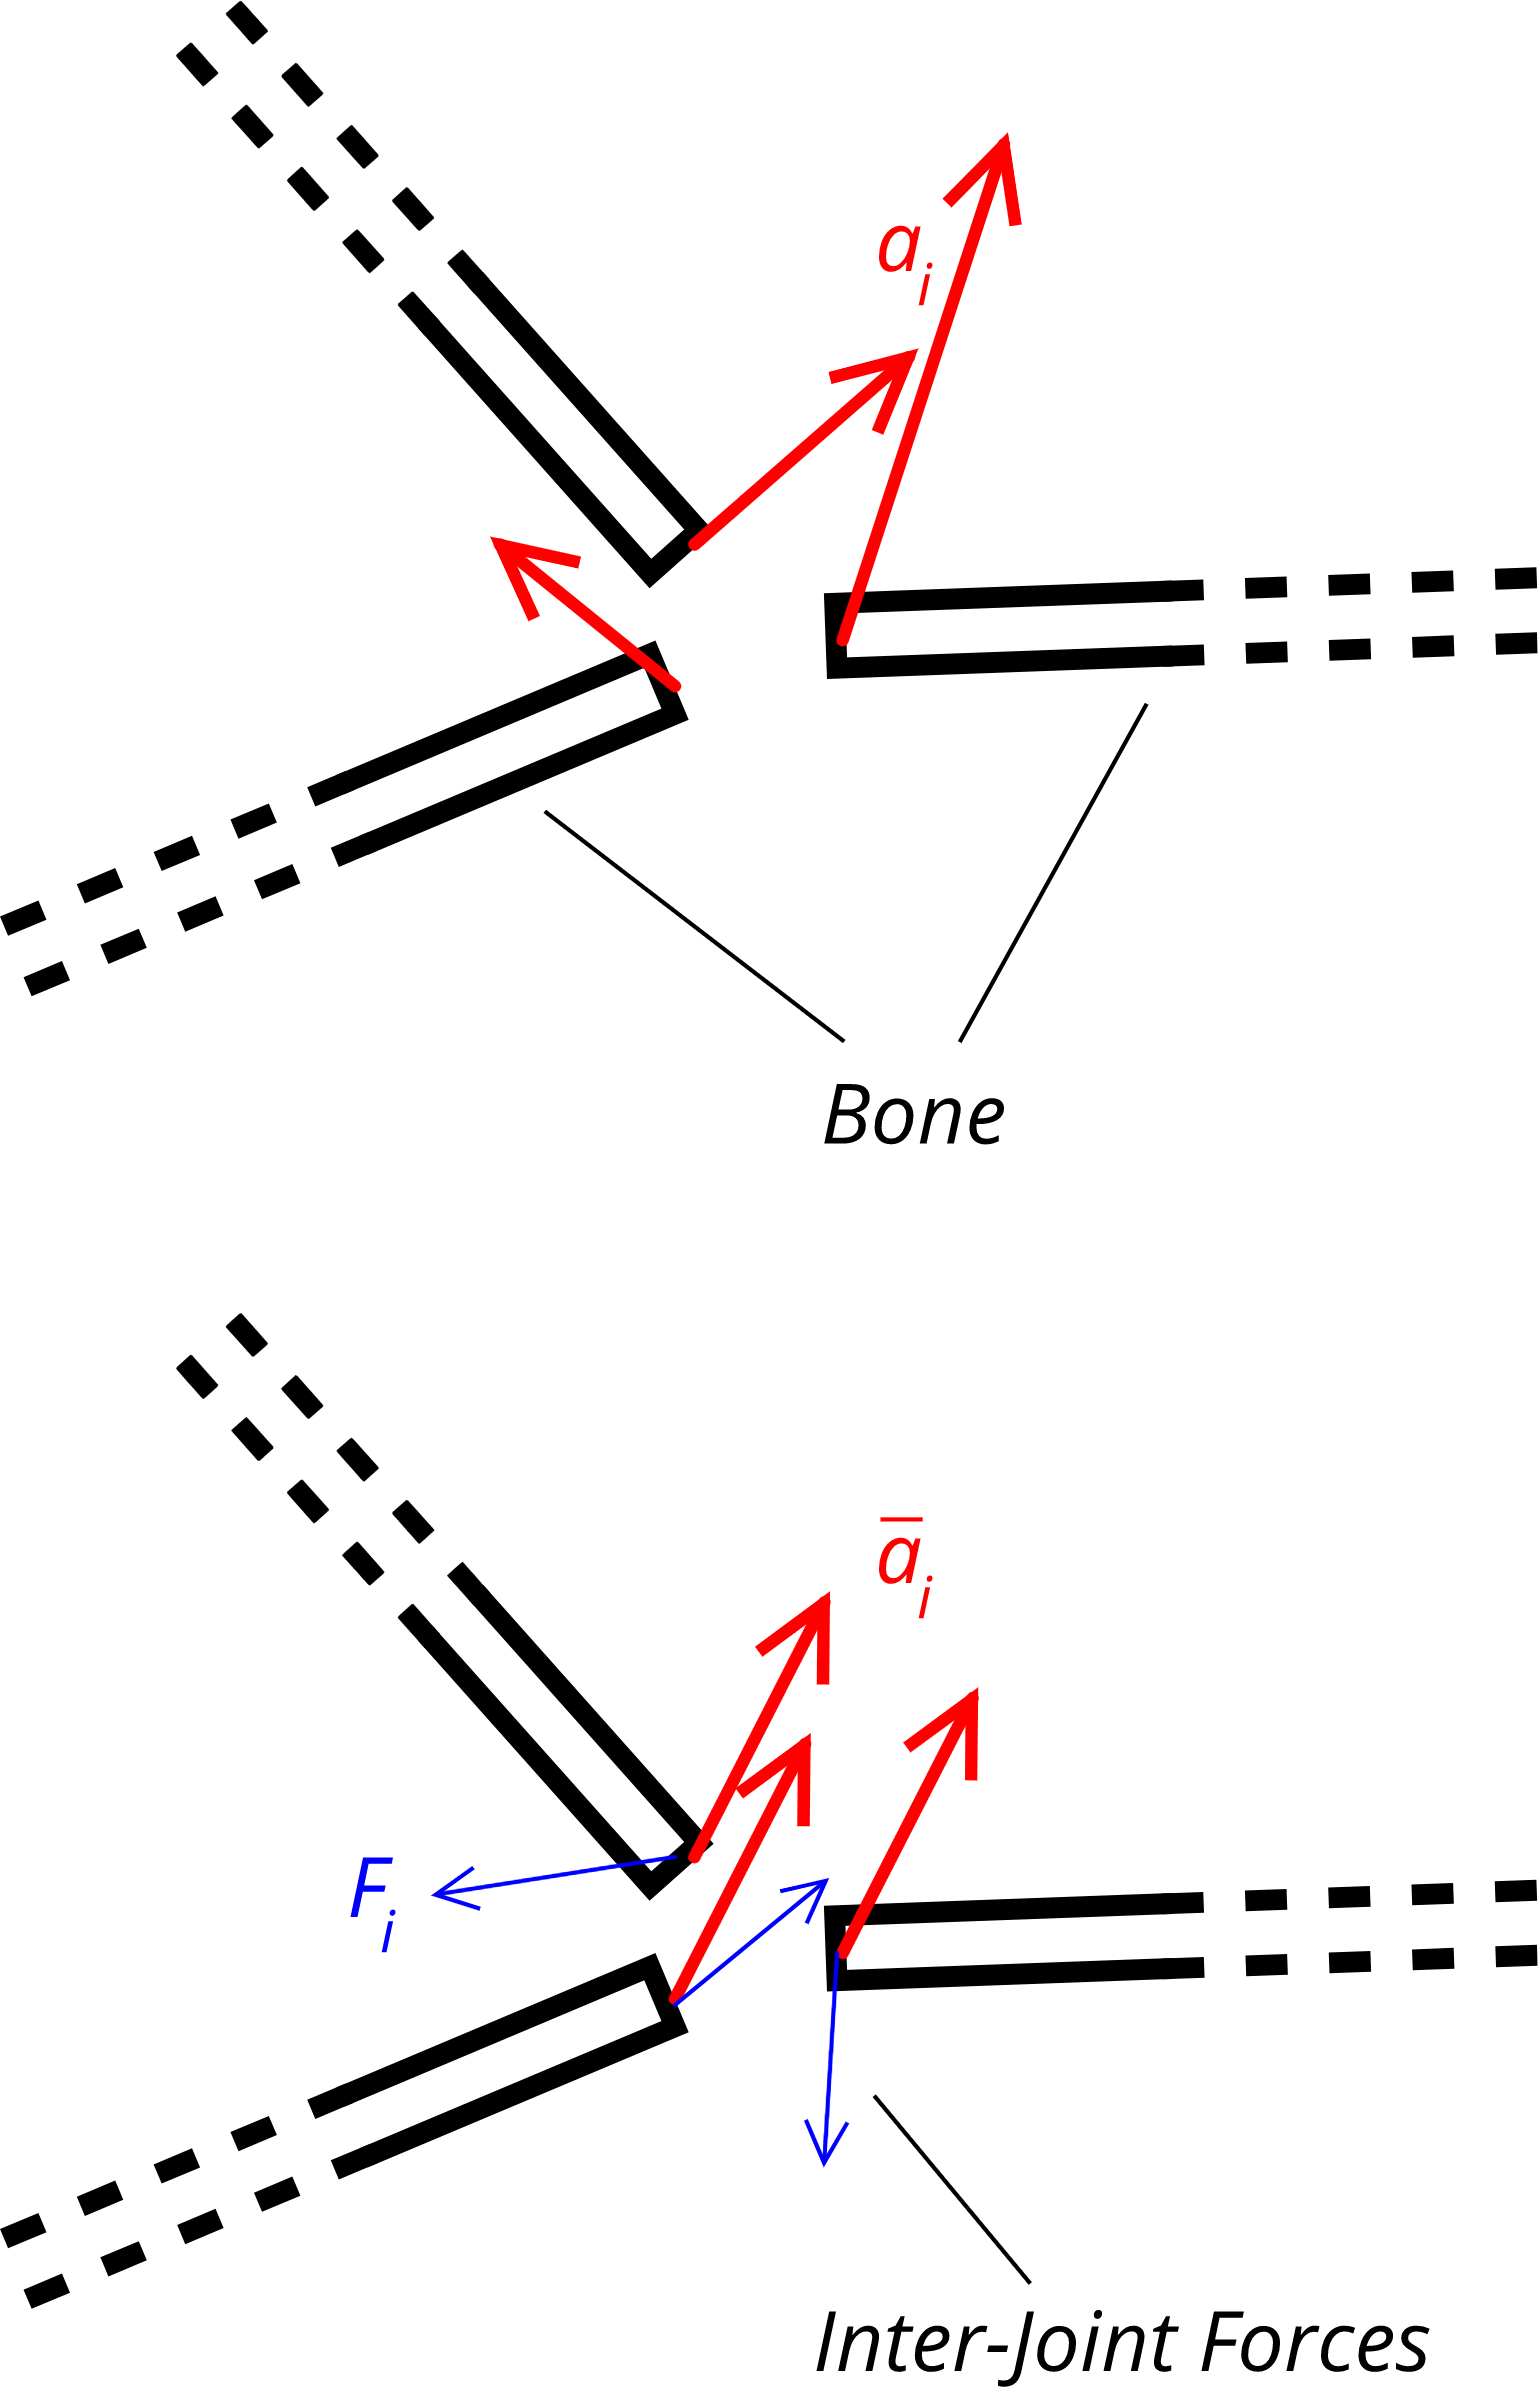
\includegraphics[width=0.7\columnwidth] {diagram2.png}
    \caption{Annotated diagram illustrating the application of inter-joint forces}
    \label{img:inter-joint}
\end{figure}

Suppose $k$ bones $B_1, B_2, ..., B_k$ are connected at a joint. The following heuristic is used to ensure that they remain connected. Inter-joint forces $F_1, F_2, ..., F_k$ are applied the corresponding bone such that:
\begin{equation}
F_1 + F_2 + ... + F_k = 0
\end{equation}
and
\begin{equation}
\bar{\bm{a}}_1 = \bar{\bm{a}}_2 = ... = \bar{\bm{a}}_k
\end{equation}
Where $\bar{\bm{a}}_1$ is the acceleration of $B_i$ at the location of the joint. Let $A_i$ be the force-acceleration matrix for $B_i$ where $\bm{r}$ is the position of the joint. Then the acceleration constraint can be expressed as follows:
\begin{equation}
A_1 F_1 = A_2 F_2 = ... = A_k F_k = \bm{v}
\end{equation}
Where $\bm{v}$ is some constant vector. Inverting each $A_i$, the term for the forces can be isolated:
\begin{equation}
F_i = A_i^{-1} \bm{v} 
\label{eq:fav}
\end{equation}
Then since the forces should sum to $\bm{0}$, the following relation is obtained.
\begin{multline}
A_1^{-1} \bm{v} + A_2^{-1} \bm{v} + ... + A_k^{-1} \bm{v} \\
= (A_1^{-1} + A_2^{-1} + ... + A_k^{-1}) \bm{v} = \bm{0} 
\end{multline}
Then $\bm{v}$ can be computed directly with the following:
\begin{equation}
\bm{v} =  (A_1^{-1} + A_2^{-1} + ... + A_k^{-1})^{-1} \bm{0}
\end{equation}
Once $\bm{v}$ is computed, the inter joint forces can be computed with eq. \ref{eq:fav}. 

This enables the computation of the inter-joint forces at a single joint after all other forces have been computed. This can be extended to simultaneously solve for all joints at once, but this would require the inversion of a large matrix. Iteratively computing the inter-joint forces at each joint approaches an approximate solution, sacrificing physical accuracy for speed and simplicity. This loss of accuracy can lead to divergent solutions, which are mitigated by control point movement interpolation in the following section.

The inter-joint forces are thus computed for each joint in multiple passes until the maximum difference in acceleration between any two bones at any joint has a magnitude less than some $\epsilon$.

\paragraph{Control point springs.} As stated before, a control point consists of a target point and an attachment point. The attachment point, which is on the rig, is brought to its target position (target point) by simulating connecting the two with rest length 0. Two types of springs were considered: linear, and capped-linear. The forces are computed as follows.

\begin{figure}[]
    \centering
    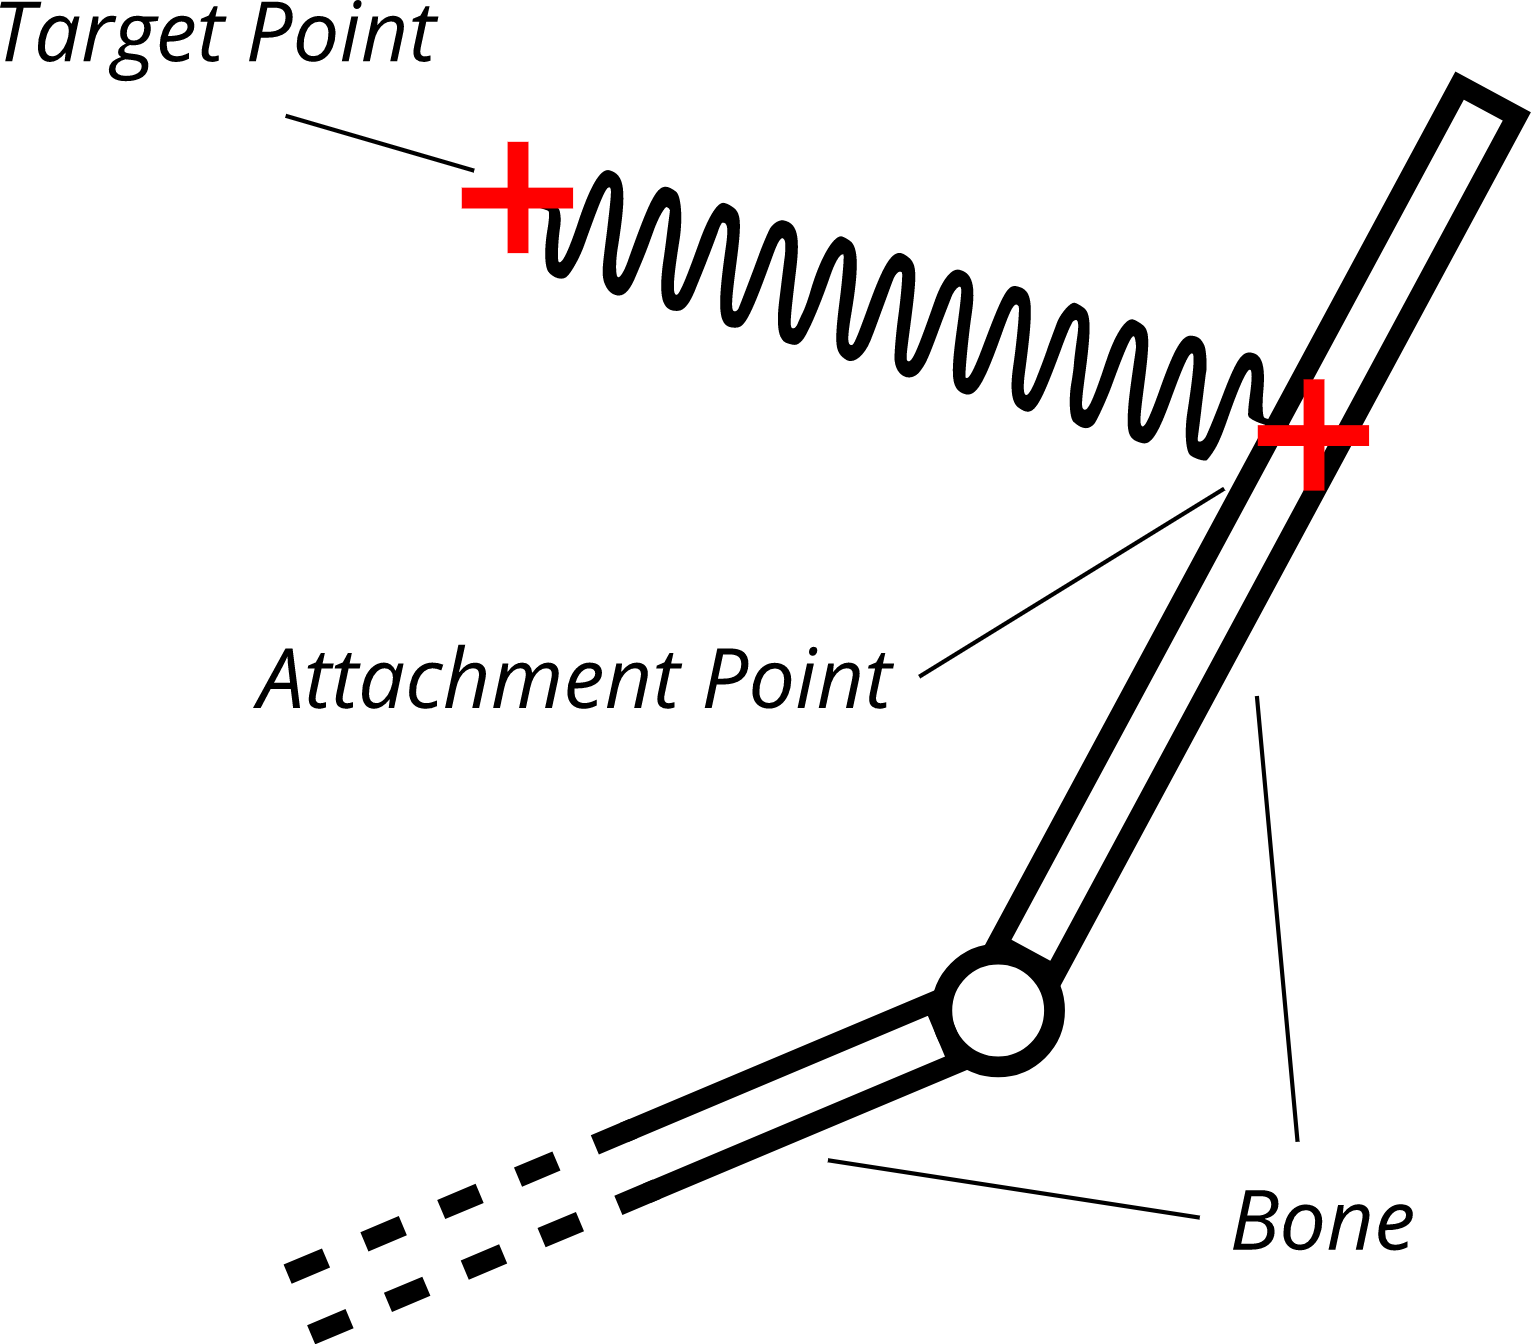
\includegraphics[width=0.7\columnwidth] {diagram1.png}
    \caption{An illustration of the spring forces in a control point system.}
    \label{img:cp-spring}
\end{figure}

Suppose $a$ is the position of the attachment point, $B$ is the specific bone on which $a$ is attached, and $t$ is the target position. A force $F$ is applied on $B$, where $F$ is defined below for different types of springs:
\begin{itemize}
    \item Linear: $F = -k(a-t)$
    \item Capped-linear: $F = -k \min(\|a - t\|, c) \left[ \frac{a-t}{\|a - t\|} \right]$
\end{itemize}
Where $k$ is the spring constant and $c$ is proportional to the maximum force of a capped-linear spring. Linear springs have the advantage that large displacements cause larger forces spring forces that move the rig into place faster. However, because the forces are unbounded, there is a potential for large forces to cause the simulation to diverge. Capped-linear springs solve this issue by placing a maximum on the force that a spring can apply. Specific examples of simulations with both types of springs are in section 4 below.

\paragraph{Torsion springs.} Torsion springs are used to enforce angular constraints. Define $y$ as the axis pointing down the bone, and let $x, z$ be the axes perpendicular to $y$ and to each other. Note that these axes are local to the bone, and change as the parent bone moves or rotates. An angular constraint may be defined for any combination of these axes and it constrains the angle at the joint where the bone meets its parent to a certain interval around each axis. 

\begin{figure}[]
    \centering
    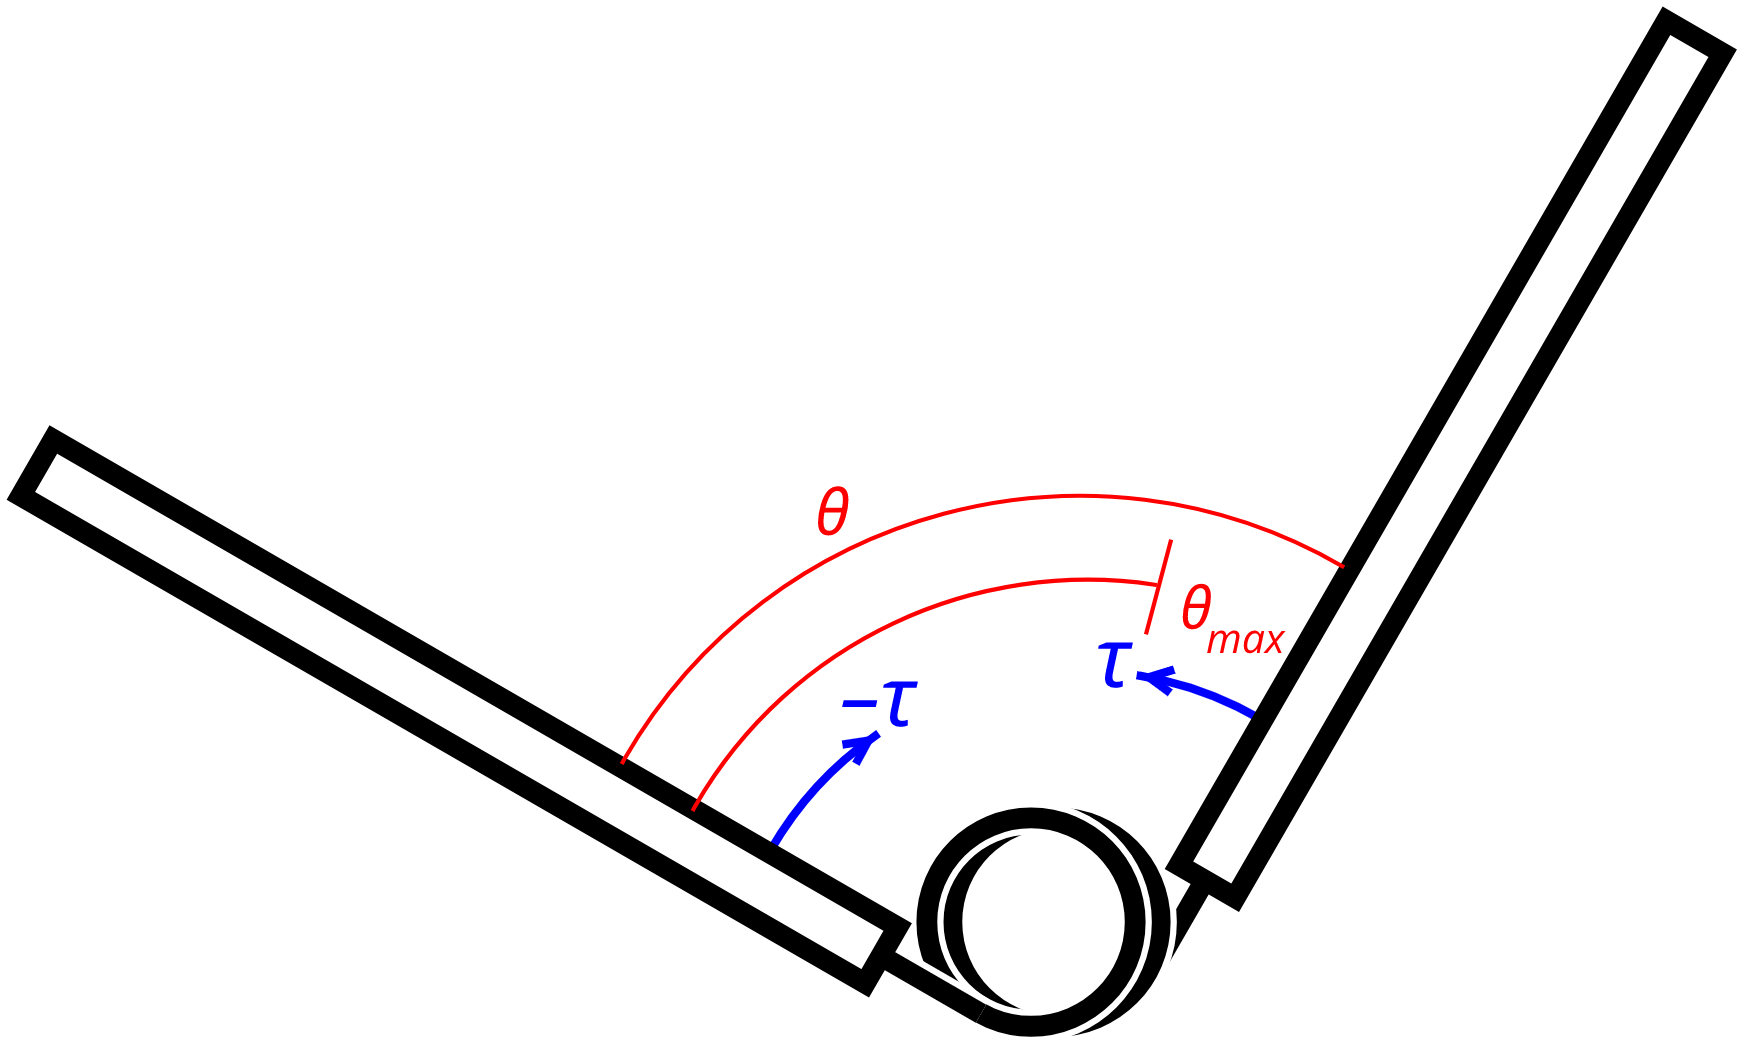
\includegraphics[width=0.7\columnwidth] {diagram6.png}
    \caption{An illustration of a joint that exceeds the maximum angle defined by an angular constraint, and the simulated corrective torque.}
    \label{img:cp-spring}
\end{figure}

Suppose the rotation at the joint some axis $\bm{v}$ is constrained to $[\theta_{min}, \theta_{max}]$, and the rotation about the $\bm{v}$ axis is currently $\theta$. Then a torque $\bm{\tau}_v$, proportional to $\bm{v}$, is applied to the bone and a torque of $-\bm{\tau}_v$ is applied to the parent bone, $\bm{\tau}_v$ is defined below for different types of springs.
\begin{itemize}
\item Linear: $\bm{\tau} = L(\theta) \bm{v} $ 

where $L(\theta) = \begin{cases} -k (\theta - \theta_{max}) & \text{if } \theta > \theta_{max} \\  -k (\theta - \theta_{min}) & \text{if } \theta < \theta_{min} \\ 0 & \text{otherwise} \end{cases}$

\item Capped-linear: $\bm{\tau} = \min(L(\theta), c) \bm{v} $ 
\end{itemize}
Where $k$ is the spring constant and $c$ is proportional to the maximum force of a capped-linear spring. This $\bm{\tau}_v$ is calculated for each axis $x, y, z$ to compute the total constraint enforcing torque of $\bm{\tau} = \bm{\tau}_x + \bm{\tau}_y + \bm{\tau}_z$, which is then applied to the bone, while $-\bm{\tau}$ is applied to the parent bone.

While capped-linear springs are more stable, they are not as good at enforcing angular constraints because they have a limit on how much torque they can output. Linear springs turn out to be stable enough while effectively enforcing angular constraints. 

\paragraph{Damping.} Damping was applied at the ends of each bone according to the usual $F_{damping} = -k \bm{v}$ where $\bm{v}$ is the velocity of the end of the bone. Angular velocity was damped by halving the angular velocity at each iteration.

\subsection{Control Point Movement}

When the user moves the target point, the actual position of the target point used in the computation of spring forces above is interpolated over a certain number of iterations, with which the rest of the simulation is run with the target point in its final position. Three schemes of interpolation were examined: linear interpolation, polar interpolation around the head of the bone, and polar interpolation around the center of mass of the rig. \\

For the following, suppose the target point was at a position $\bm{t}_{old}$ and was moved to the position $\bm{t}_{new}$. Also, suppose the number of iterations to run is $i_{max}$. Let $\bm{t}_i$ be the position of the target point used in spring force computation at the $i$-th iteration.

\paragraph{Linear Interpolation.} The linear interpolation method simply moves the effective position of the target point in a straight line from $\bm{t}_{old}$ to $\bm{t}_{new}$ at constant speed. Then $t_i$ be computed by the following formula:
\[ t_i = t_{old} \left( 1 - \frac{i}{i_{max}} \right) + t_{new} \left( \frac{i}{i_{max}} \right) \]

\paragraph{Polar Interpolation.} This method moves the effective position of a target point in an arc around the origin of rotation. The origin of rotation, which could be the head of the bone of the center of mass of the rig, may change at each iteration. The angle between the interpolated target position and the new target position (with the origin as the pivot) is varied at a constant rate, while the distance from the interpolated target position is also varied at a constant rate until it matches the distance from the new target position and the origin.

This is formulated mathematically as follows. Let $\bm{o}_i$ be the origin of rotation at iteration $i$.  Then $\bm{t}_i$ can be described by the following recurrence relation:
\begin{equation}
    \begin{aligned}
    \bm{t}_0 &= \bm{t}_{old} \\
    \bm{t}_{i+1} &= r_i R(\bm{n}_i, \alpha_i \theta_i) \frac{ \bm{t}_i - \bm{o}_i } { \| \bm{t}_i - \bm{o}_i \| } + \bm{o}_i
    \end{aligned}
\end{equation}
where 
\begin{align*}
\bm{n}_i &= \text{the vector normal to } \bm{t}_i - \bm{o}_i \text{ and } \bm{t}_{new} - \bm{o}_i \\
\theta_i &= \text{the angle between } \bm{t}_i - \bm{o}_i \text{ and } \bm{t}_{new} - \bm{o}_i \\
R(\bm{n}_i, \theta_i) &= \text{rotation by an angle } \theta_i \text{ about the axis } \bm{n}_i 
\end{align*}
and
\begin{align*}
    \alpha_i &= \frac{1}{i_{max} - i} \\
    r_i &= (1 - \alpha_i) \| \bm{t}_i - \bm{o}_i \| + \alpha_i \| \bm{t}_{new} - \bm{o}_i \| 
\end{align*} 

To avoid dividing by 0, if either $\bm{t}_i$ or $\bm{t}_{new}$ is too close to $\bm{o}_i$, then the algorithm falls back on linear interpolation.

\section{Results}

\begin{figure}[]
    \centering
    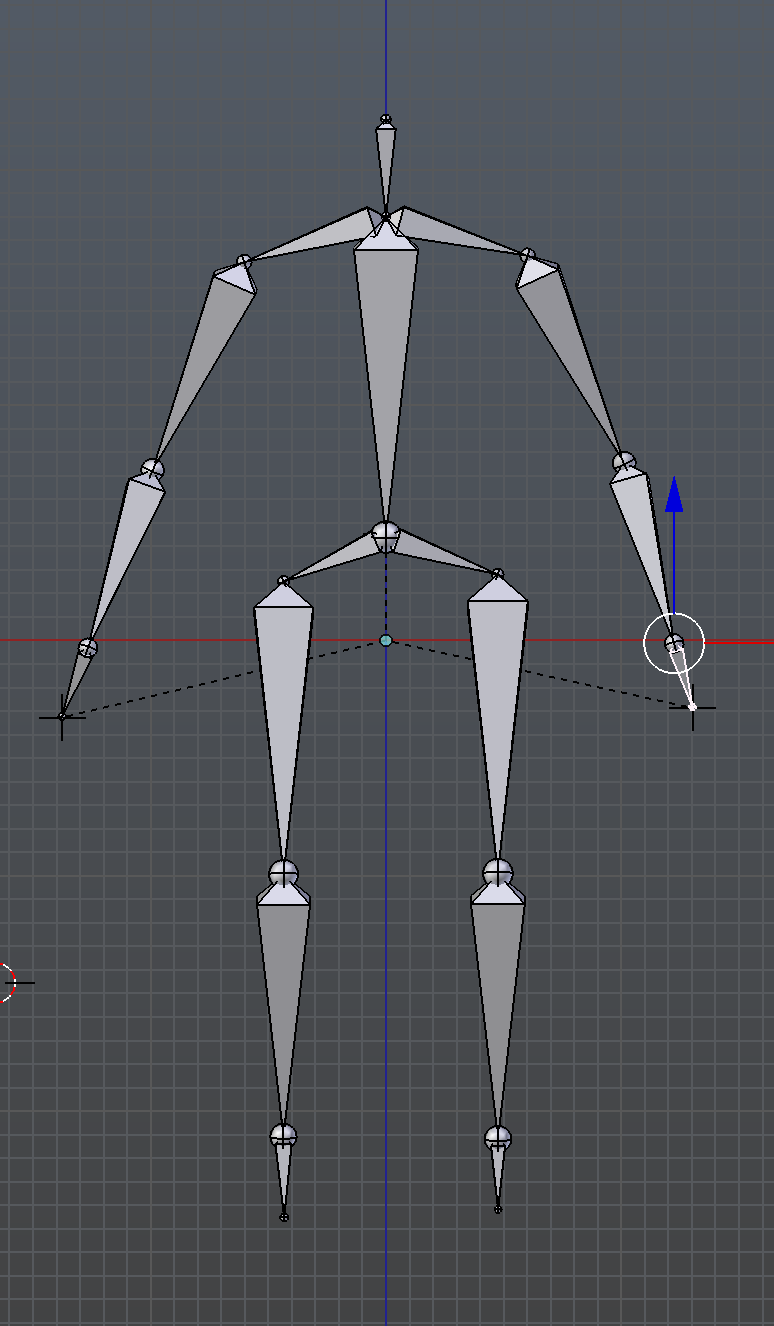
\includegraphics[width=0.7\columnwidth] {pinhead.png}
    \caption{The rig used to evaluate the performance of PhysIK.}
    \label{img:pinhead}
\end{figure}

The rig in figure \ref{img:pinhead} was the primary test case used to evaluate the performance of PhysIK on the objectives outlined above. It consists of 18 bones and 14 joints, with a maximum of 4 bones around a single joint. The angle between the torso, the collarbone and hips are fixed with 0 degrees of freedom. The elbow and the knees have one degree of freedom and are constrained between 0 (straight out) and 120 degrees on the axis perpendicular to the length of the bone, and fixed on the axis parallel. The head, hip, and shoulder joints have 3 degrees of freedom and are unconstrained.

In each of the following examples, the $\Delta t$ used to step the simulation was 0.05, with a damping coefficient of 20, and a joint acceleration epsilon of $0.001$ (in arbitrary Blender units). 

\begin{figure}[]
    \centering
    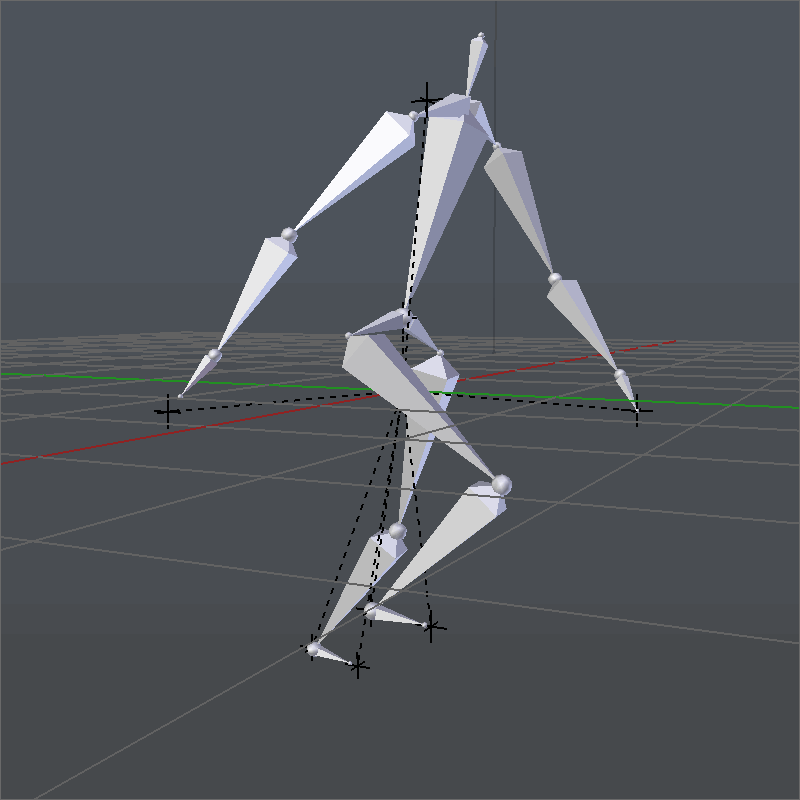
\includegraphics[width=0.7\columnwidth] {pose-frame.png}
    \caption{A static running pose.}
    \label{img:running}
\end{figure}

\paragraph{Accuracy.} Figure \ref{img:running} is a screenshot of a static pose created using PhysIK. The 8 control points used to create this pose all have spring coefficients of 30.

Observe that rig coincides with the control points on the right hand and on the feet. The control points on the left hand and shoulder are visibly out of place, but notice that they are too far apart to make a feasible pose. This highlights the fact that PhysIK can still produce good results even when the constraints are impossible to satisfy. 

\begin{figure}
    \centering
    \begin{subfigure}{0.5\columnwidth}
        \centering
        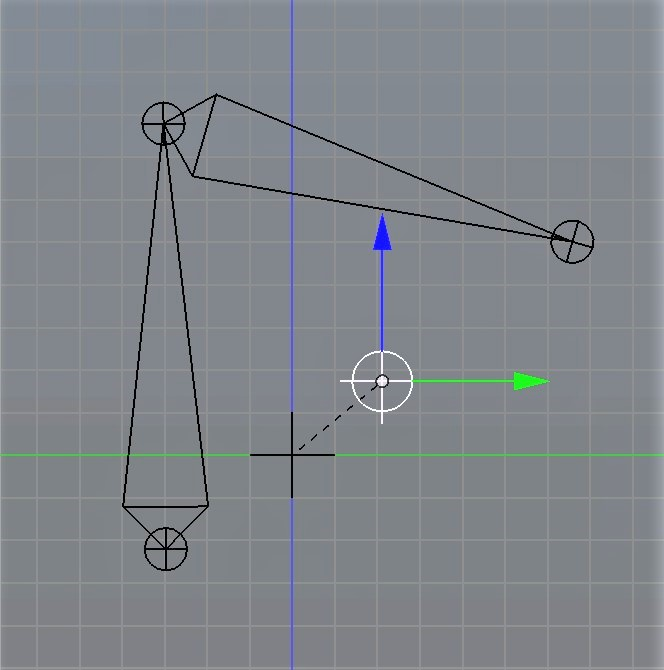
\includegraphics[width=.8\linewidth]{linear-elbow.jpg}
    \end{subfigure}\begin{subfigure}{0.5\columnwidth}
        \centering
        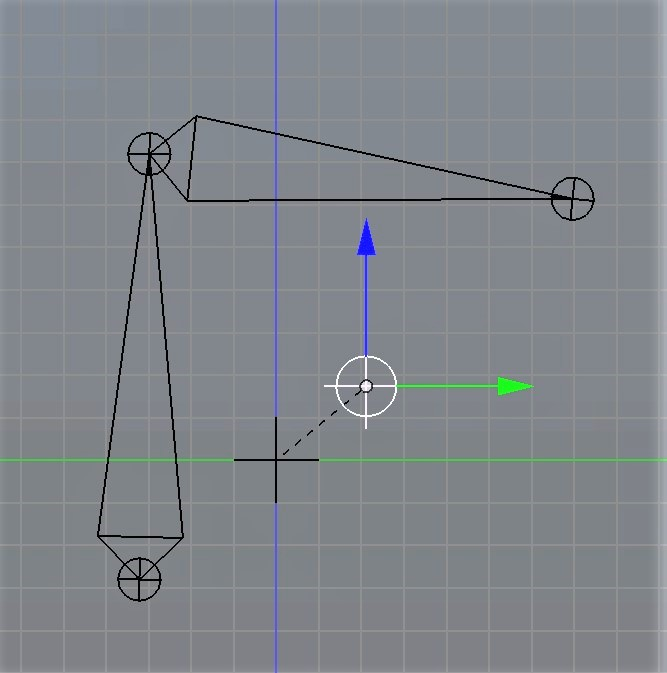
\includegraphics[width=.8\linewidth]{capped-elbow.jpg}
    \end{subfigure}

    \caption{A comparison of linear (left) and capped-linear (right) springs on an elbow constrained to 90°.}
    \label{img:elbow}
\end{figure}

For a comparison of accuracy on linear and capped-linear springs, two examples were used. First, to evaluate the accuracy of angular constraints, consider figure \ref{img:elbow}. The rig in the figure is a simple elbow rig, where the angle between the bones is constrained between $180\degree$ and $90\degree$. Note that the configuration defined by the control points is impossible to reach without breaking angular angular constraints. What is of significance here is the degree to which the angular constraints are broken. A linear spring puts more stress on the torsion spring enforcing the angular constraint than the capped linear spring would, resulting in a joint that is clearly overbent.

Another aspect of accuracy can be seen in the next example with linear and capped-linear springs. When the control point is instantly moved to a point far away, the simulation initially diverges for the linear spring, and converges to a strange pose, especially near the elbow and hips (see figure \ref{img:cannon}). When capped linear springs are used, the algorithm converges to stably, though it takes a few more iterations.

\begin{figure*}
    \centering
    \begin{subfigure}{0.2\textwidth}
        \centering
        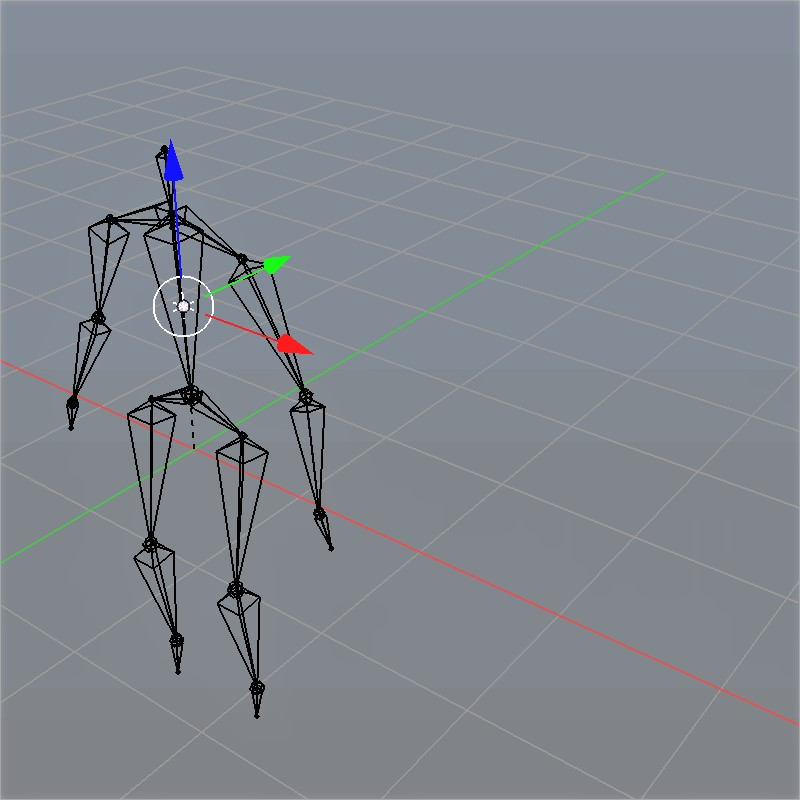
\includegraphics[width=.9\linewidth]{linear-cannon-0.jpg}
        \caption{step 0, $t=0$ms}
    \end{subfigure}\begin{subfigure}{0.2\textwidth}
        \centering
        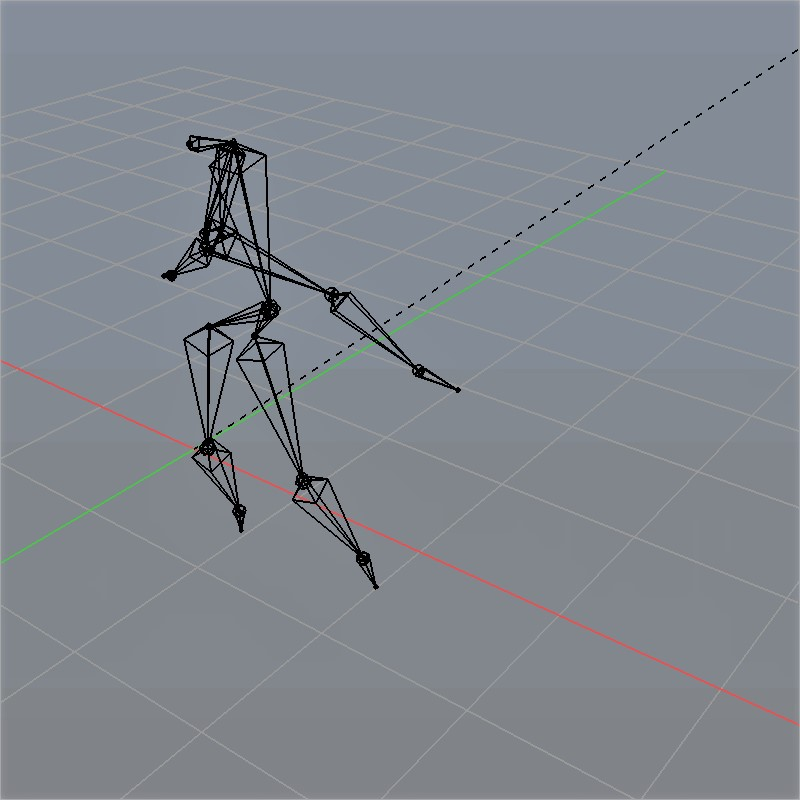
\includegraphics[width=.9\linewidth]{linear-cannon-5.jpg}
        \caption{step 1, $t=5$ms}
    \end{subfigure}\begin{subfigure}{0.2\textwidth}
        \centering
        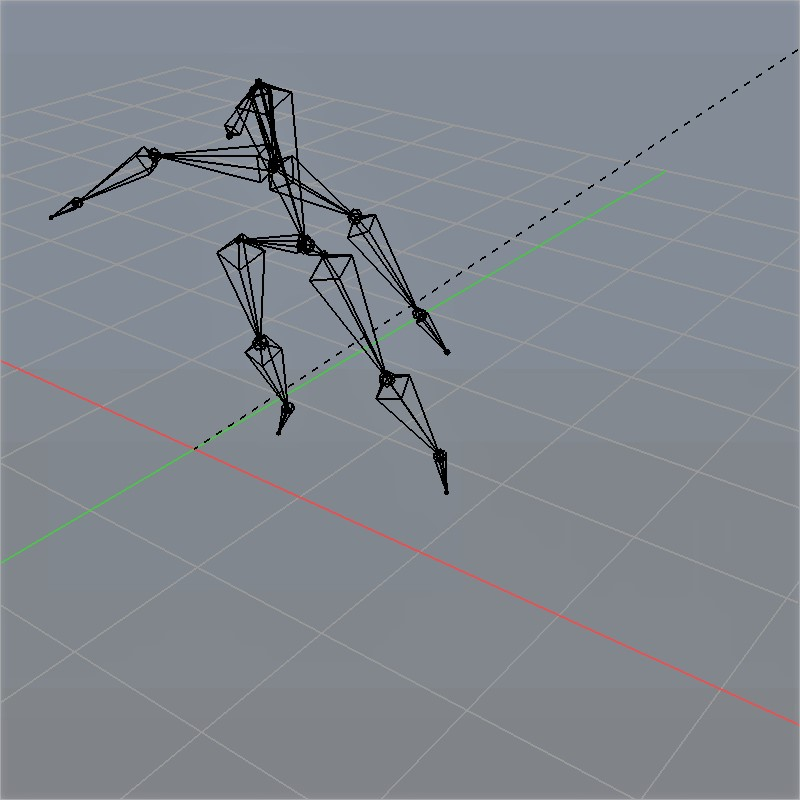
\includegraphics[width=.9\linewidth]{linear-cannon-50.jpg}
        \caption{step 10, $t=50$ms}
    \end{subfigure}\begin{subfigure}{0.2\textwidth}
        \centering
        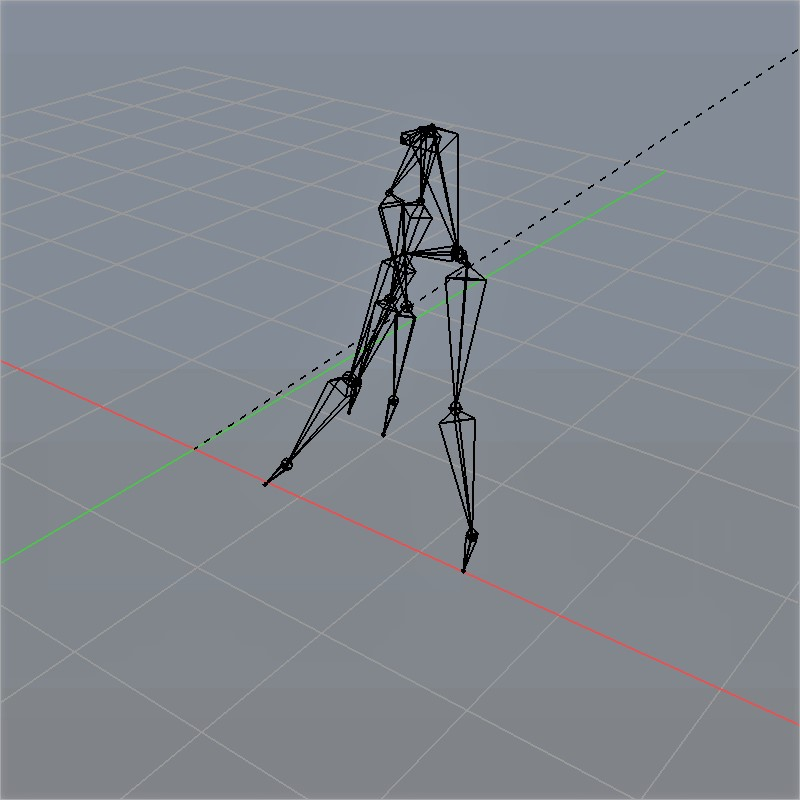
\includegraphics[width=.9\linewidth]{linear-cannon-500.jpg}
        \caption{step 100, $t=500$ms}
    \end{subfigure}\begin{subfigure}{0.2\textwidth}
        \centering
        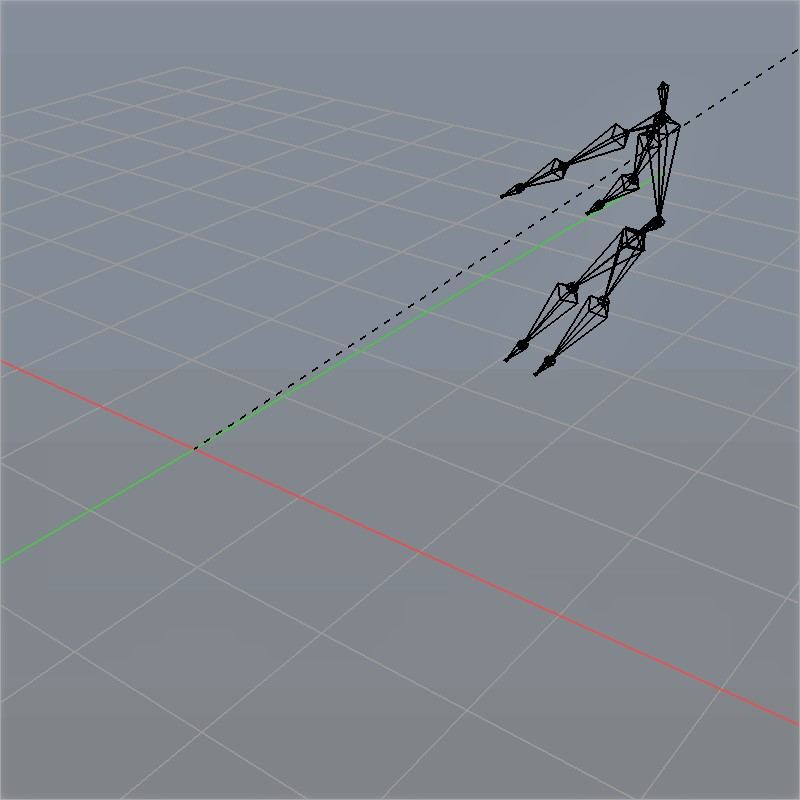
\includegraphics[width=.9\linewidth]{linear-cannon-1000.jpg}
        \caption{step 200, $t=1000$ms}
    \end{subfigure}

    \begin{subfigure}{0.2\textwidth}
        \centering
        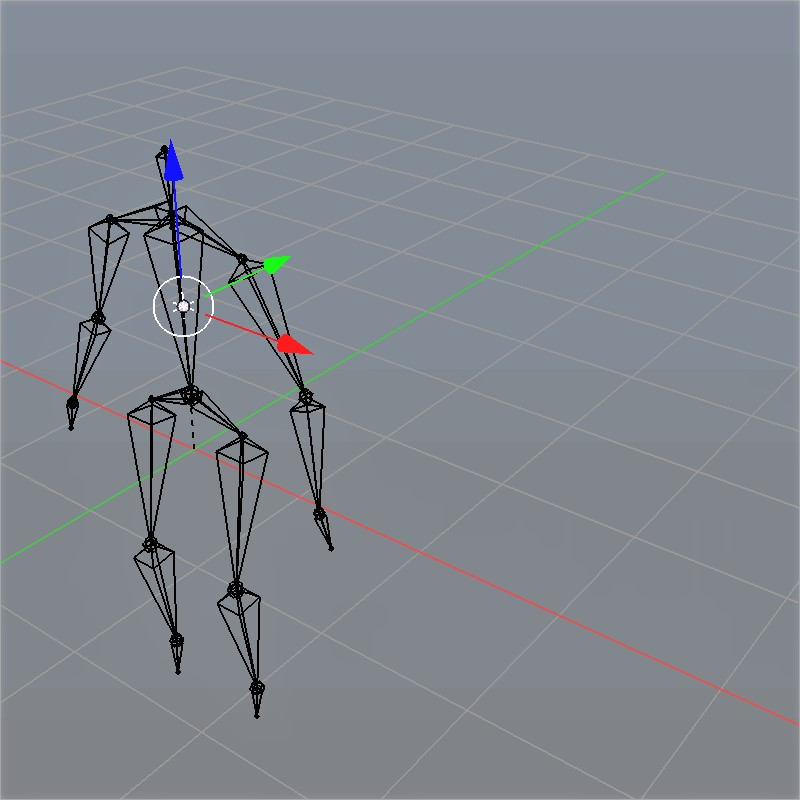
\includegraphics[width=.9\linewidth]{linear-cannon-0.jpg}
    \end{subfigure}\begin{subfigure}{0.2\textwidth}
        \centering
        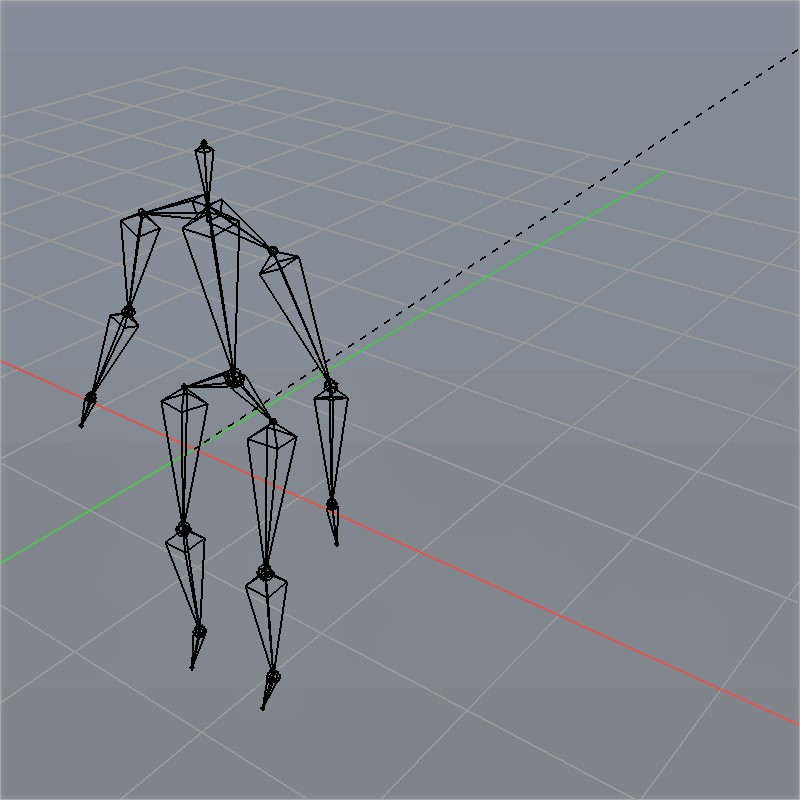
\includegraphics[width=.9\linewidth]{capped-cannon-5.jpg}
    \end{subfigure}\begin{subfigure}{0.2\textwidth}
        \centering
        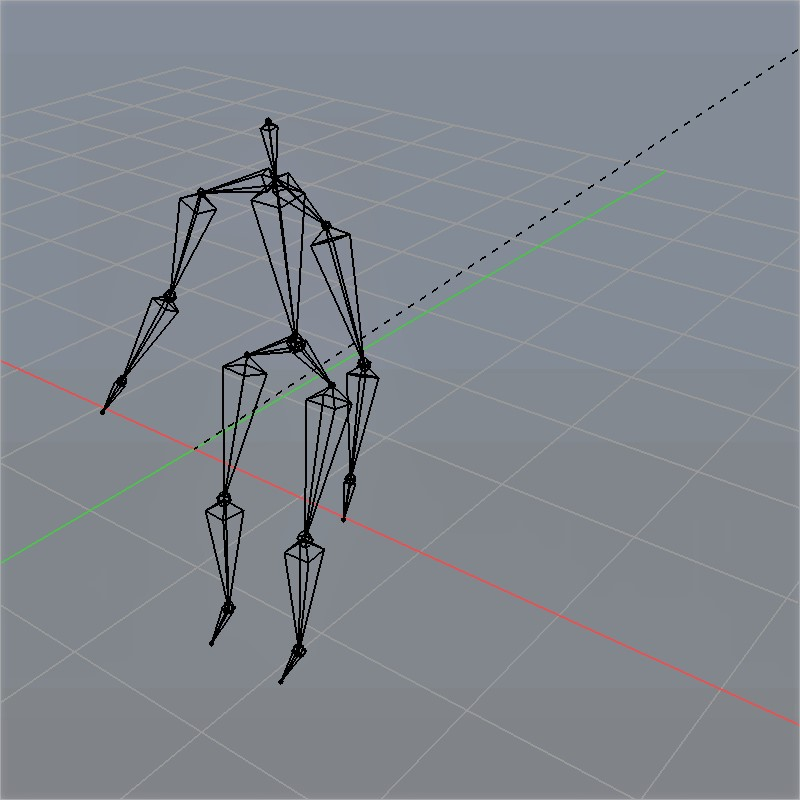
\includegraphics[width=.9\linewidth]{capped-cannon-50.jpg}
    \end{subfigure}\begin{subfigure}{0.2\textwidth}
        \centering
        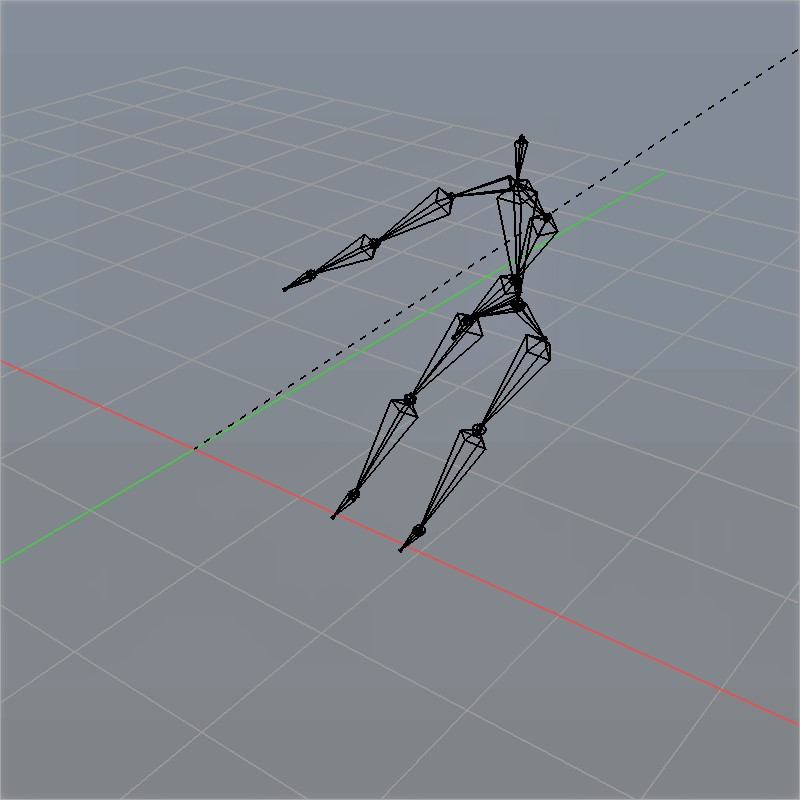
\includegraphics[width=.9\linewidth]{capped-cannon-500.jpg}
    \end{subfigure}\begin{subfigure}{0.2\textwidth}
        \centering
        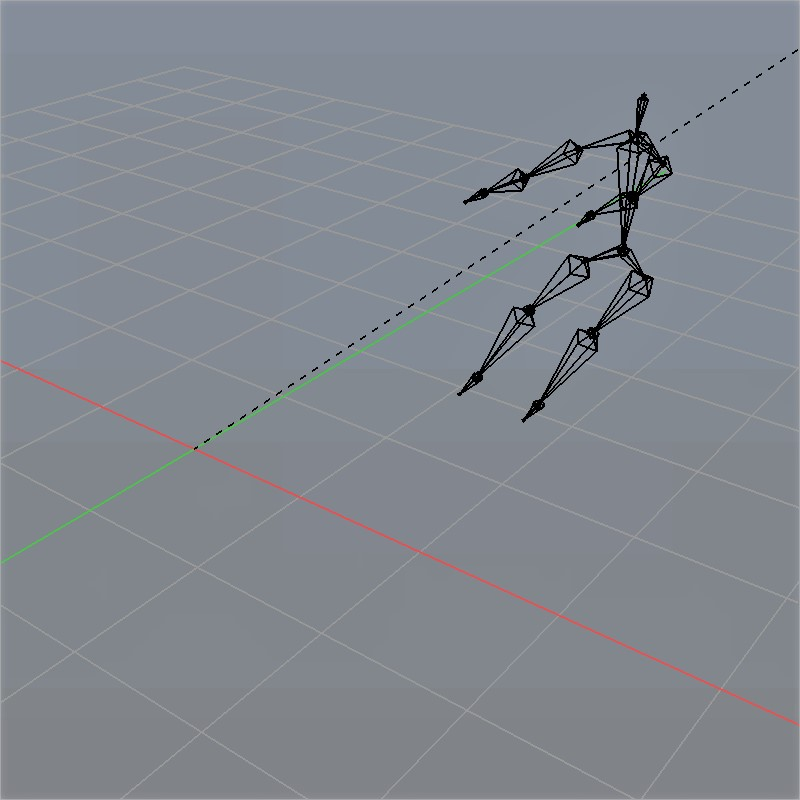
\includegraphics[width=.9\linewidth]{capped-cannon-1000.jpg}
    \end{subfigure}

    \caption{A comparison of linear (top row) and capped-linear (bottom row) springs with a large, sudden displacement of a control point.}
    \label{img:cannon}
\end{figure*}

There are cases, however, where the algorithm fails to converge entirely. When angular constraints are stressed and one of the bones in the chain have enough degrees of freedom, then oscillation can occur around the control point. For example, in figure \ref{img:wobble}, the tip of the hand will oscillate around the target point indefinitely. This is most likely caused by the inaccuracies of Euler integration combined with the extra degrees of freedom that allows for such behavior.

\begin{figure}[]
    \centering
    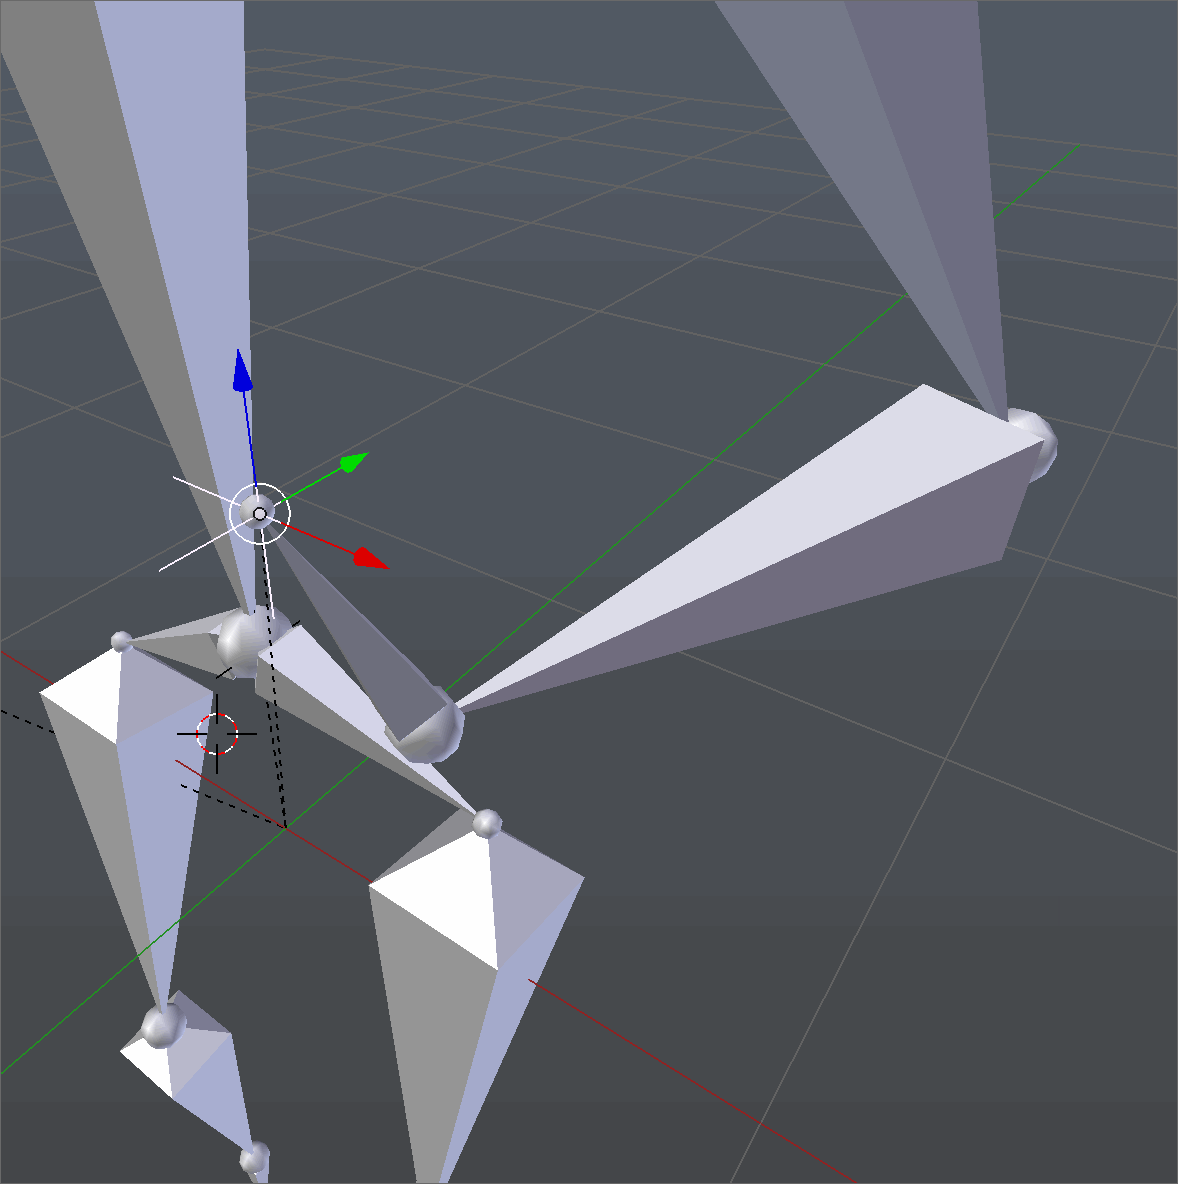
\includegraphics[width=0.7\columnwidth] {wobble-frame.png}
    \caption{A configuration where the tip of the hand oscillates around the target point.}
    \label{img:wobble}
\end{figure}

\paragraph{Interactivity.} The poses above were created starting with the pose in figure \ref{img:pinhead}, then adding and manipulating control points. The pose in figure \ref{img:running} was completed in under a minute, with the simulation converging than 3 seconds whenever a control point was moved to its target position.

When using the profile module in Python\textsuperscript{\cite{Pr}} to evaluate the speed of the algorithm, it reported an average of $\sim 98$ms per frame for the humanoid rig, with $\sim 70$ms spent on computing inter-joint forces, with around $\sim 20$ passes per step. 

The rig is simulated live while posing the rig, which makes it easier to see how the rig will move into place. It also leaves the overhead of deciding how many iterations to run to the user (i.e. it runs until the user deems that the system has converged enough). While this may not be ideal (see discussion), it also helps to hide the relatively long running time per step. When run at 100ms per frame, the tool still feels smooth enough and fast enough to use practically.

\paragraph{Intuitiveness.} Intuitiveness is difficult to measure quantitatively and is up to the preference of the user. Presented below figure \ref{img:hand} are comparisons of Blender's iTasC solver with the PhysIK algorithm on a pose with a single outstretched hand. The angular constraints are the same in both cases, and both have 3 points to specify the position of the rig. Note how the shoulder in the PhysIK pose is turned toward the viewer, and the character is leaning slightly forward. As a bonus, the head also has a slight tilt. Compare this to the stiff pose computed by Blender's iTasC solver. 

\begin{figure}
    \centering
    \begin{subfigure}{\columnwidth}
        \centering
        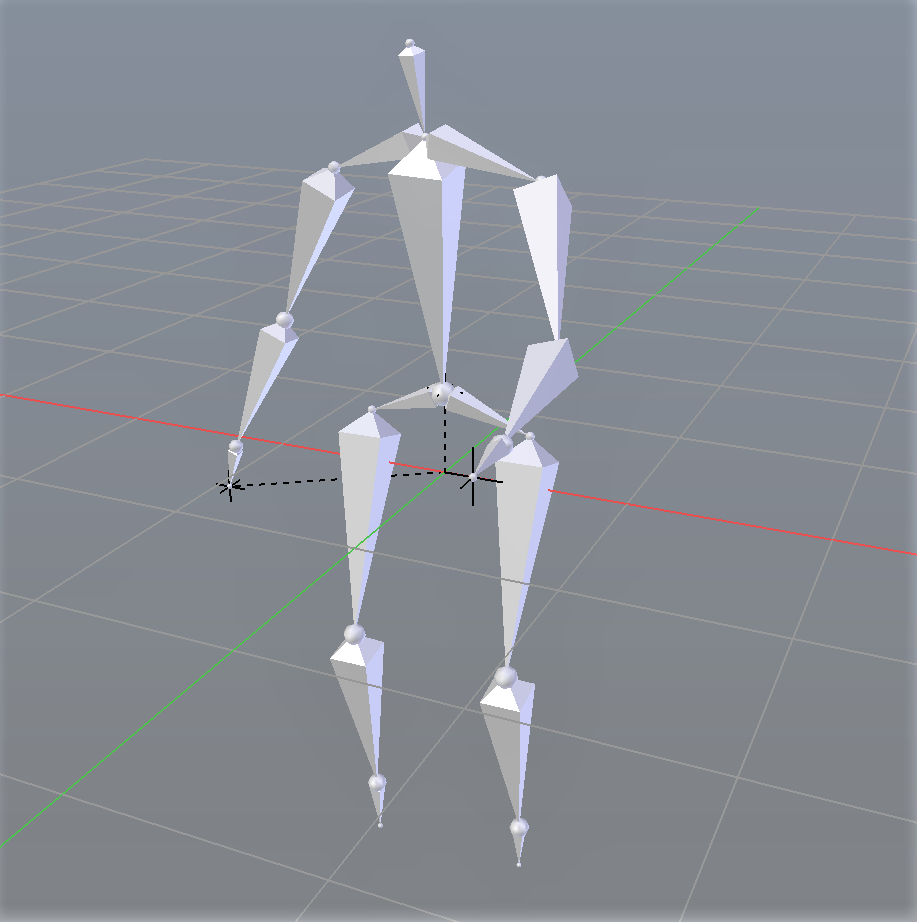
\includegraphics[width=.8\linewidth]{pose-hand.png}
    \end{subfigure}
    
    \begin{subfigure}{\columnwidth}
        \centering
        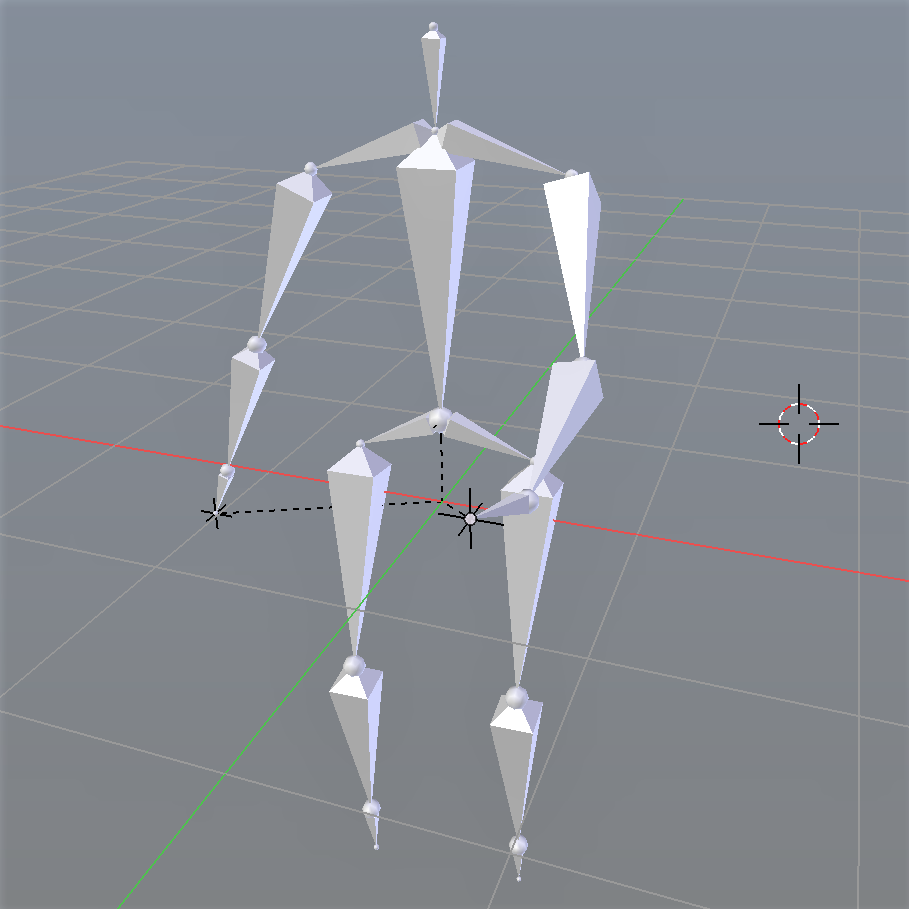
\includegraphics[width=.8\linewidth]{pose-hand-itasc.png}
    \end{subfigure}

    \caption{A comparison of PhysIK (top) and iTasC (bottom) on a pose with an outstretched hand.}
    \label{img:hand}
\end{figure}

To see how control point interpolation affects the results, consider the following set of frames. Figure \ref{img:raise} compares polar interpolation about the center of mass and linear interpolation. The control point is interpolated for the first 50 steps (250ms) and the rest is simulated normally. Note how the linear interpolation causes more secondary motion while the circular arc, which would be a more natural path for the arm, results in a more natural looking pose.

\begin{figure*}[h]
    \centering
    \begin{subfigure}{0.2\textwidth}
        \centering
        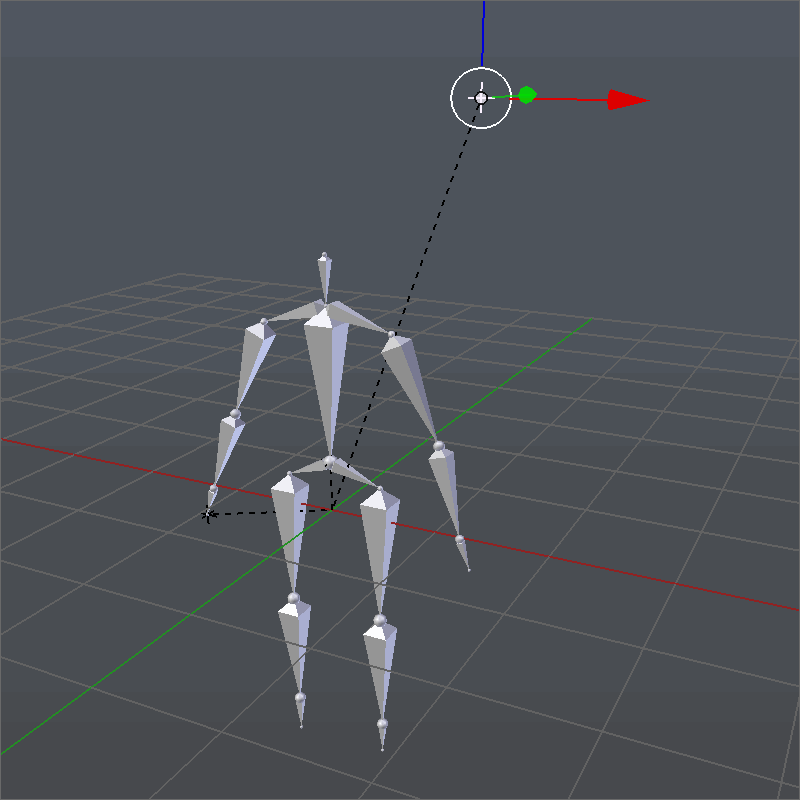
\includegraphics[width=.9\linewidth]{raise-circ-0.png}
        \caption{step 0, $t=0$ms}
    \end{subfigure}\begin{subfigure}{0.2\textwidth}
        \centering
        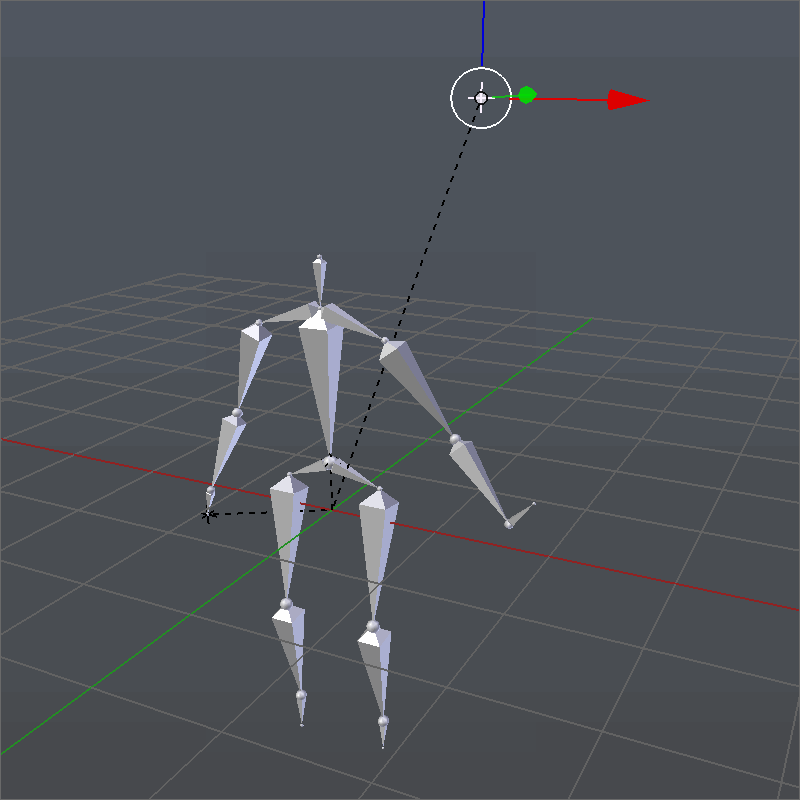
\includegraphics[width=.9\linewidth]{raise-circ-1.png}
        \caption{step 20, $t=100$ms}
    \end{subfigure}\begin{subfigure}{0.2\textwidth}
        \centering
        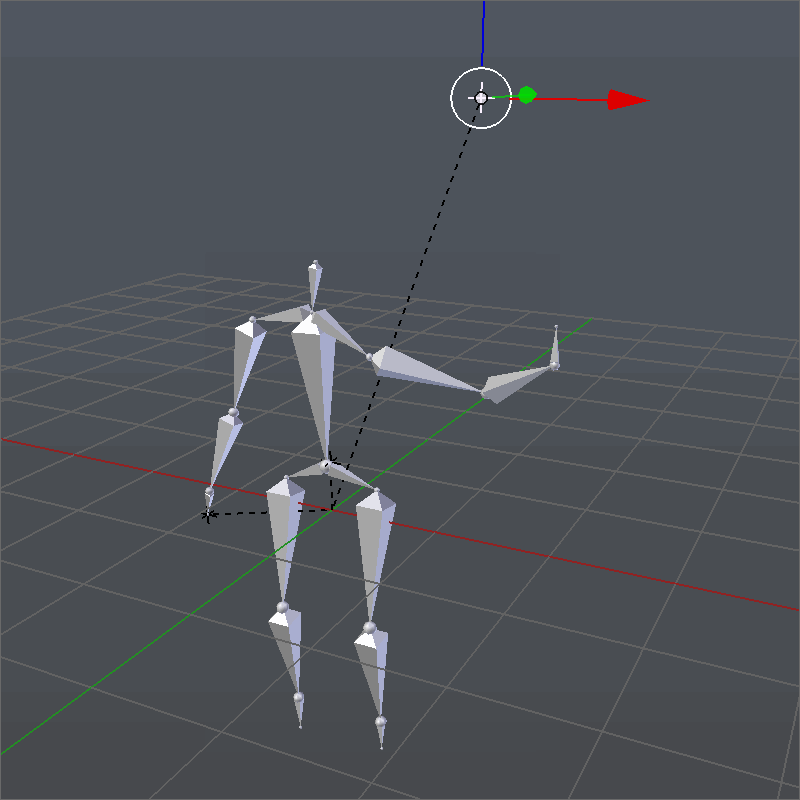
\includegraphics[width=.9\linewidth]{raise-circ-2.png}
        \caption{step 40, $t=200$ms}
    \end{subfigure}\begin{subfigure}{0.2\textwidth}
        \centering
        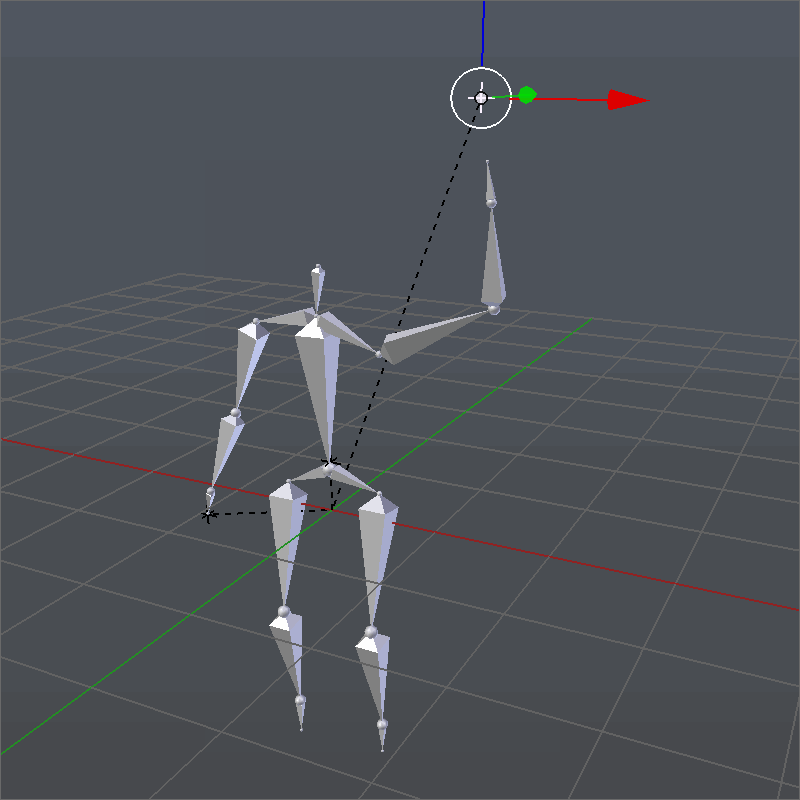
\includegraphics[width=.9\linewidth]{raise-circ-3.png}
        \caption{step 60, $t=300$ms}
    \end{subfigure}\begin{subfigure}{0.2\textwidth}
        \centering
        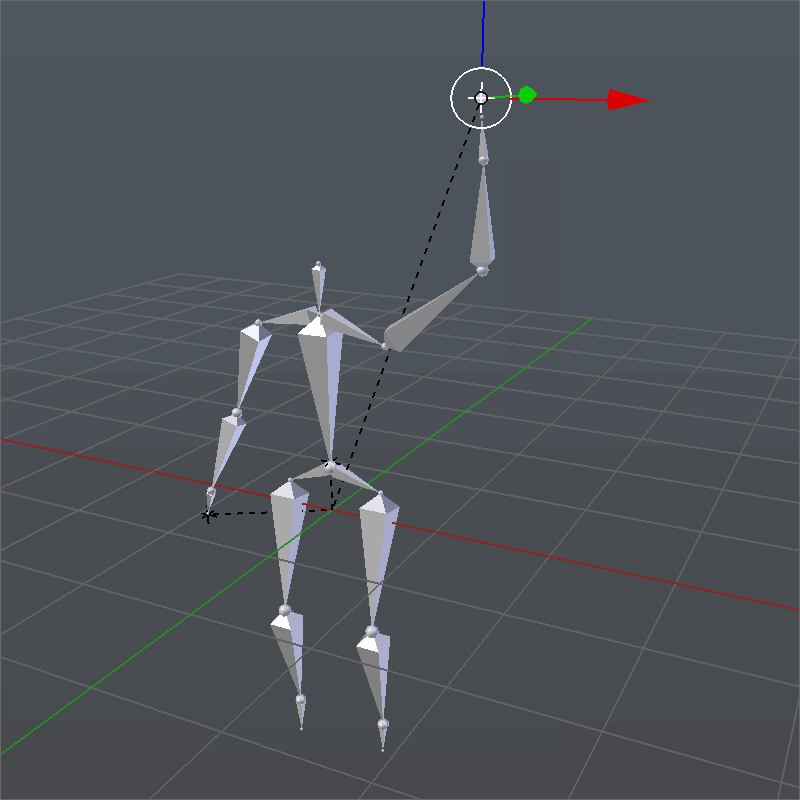
\includegraphics[width=.9\linewidth]{raise-circ-4.png}
        \caption{step 80, $t=400$ms}
    \end{subfigure}

    \begin{subfigure}{0.2\textwidth}
        \centering
        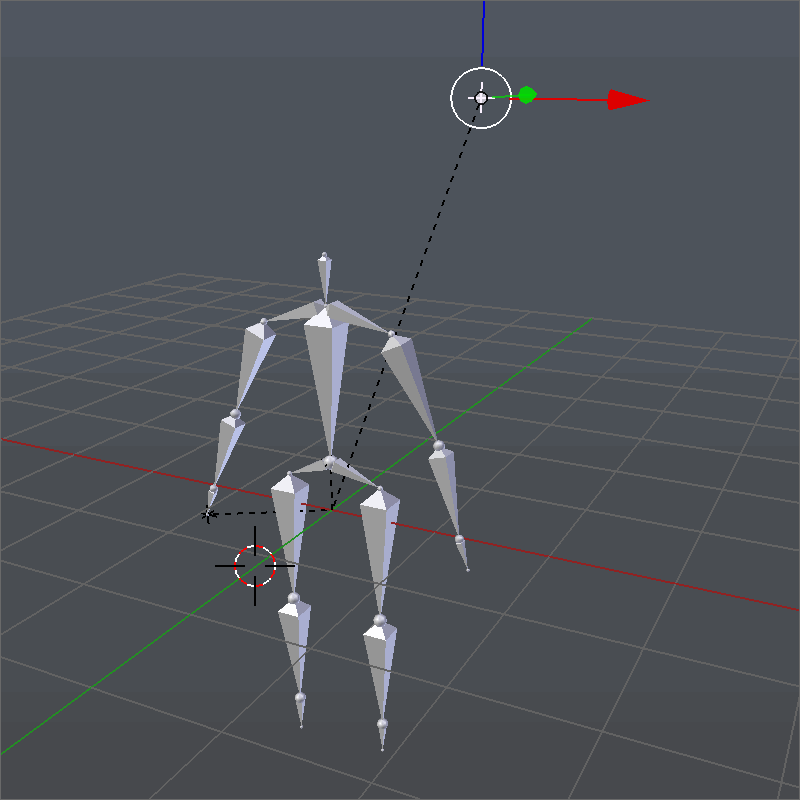
\includegraphics[width=.9\linewidth]{raise-linear-0.png}
    \end{subfigure}\begin{subfigure}{0.2\textwidth}
        \centering
        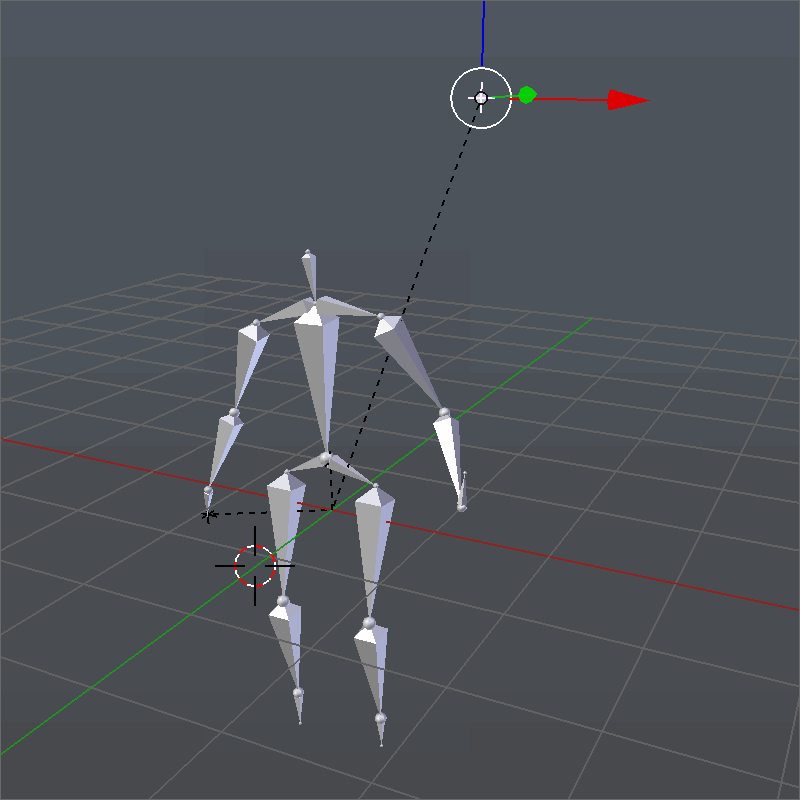
\includegraphics[width=.9\linewidth]{raise-linear-1.png}
    \end{subfigure}\begin{subfigure}{0.2\textwidth}
        \centering
        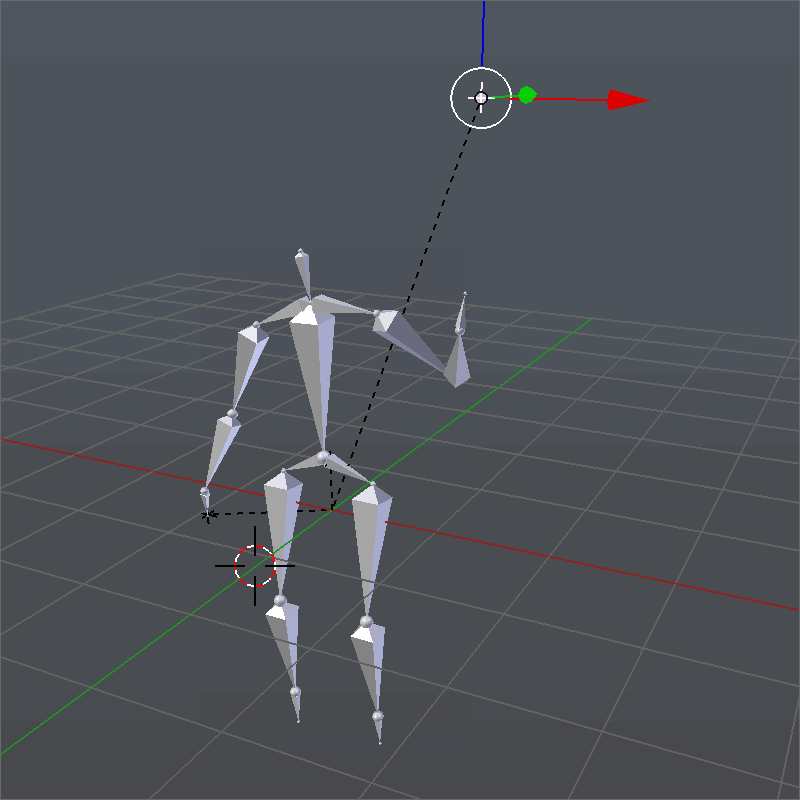
\includegraphics[width=.9\linewidth]{raise-linear-2.png}
    \end{subfigure}\begin{subfigure}{0.2\textwidth}
        \centering
        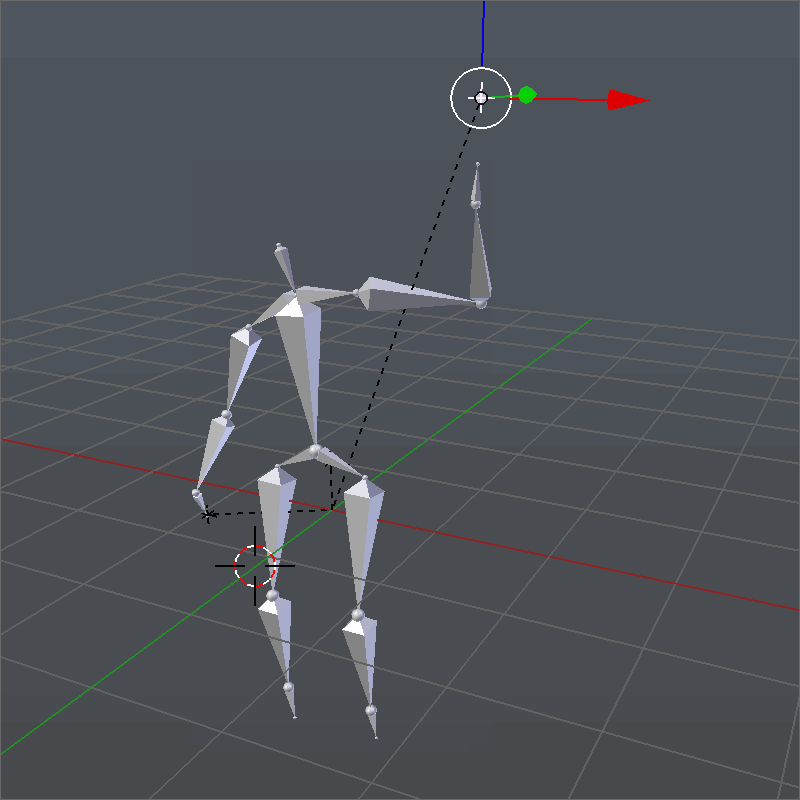
\includegraphics[width=.9\linewidth]{raise-linear-3.png}
    \end{subfigure}\begin{subfigure}{0.2\textwidth}
        \centering
        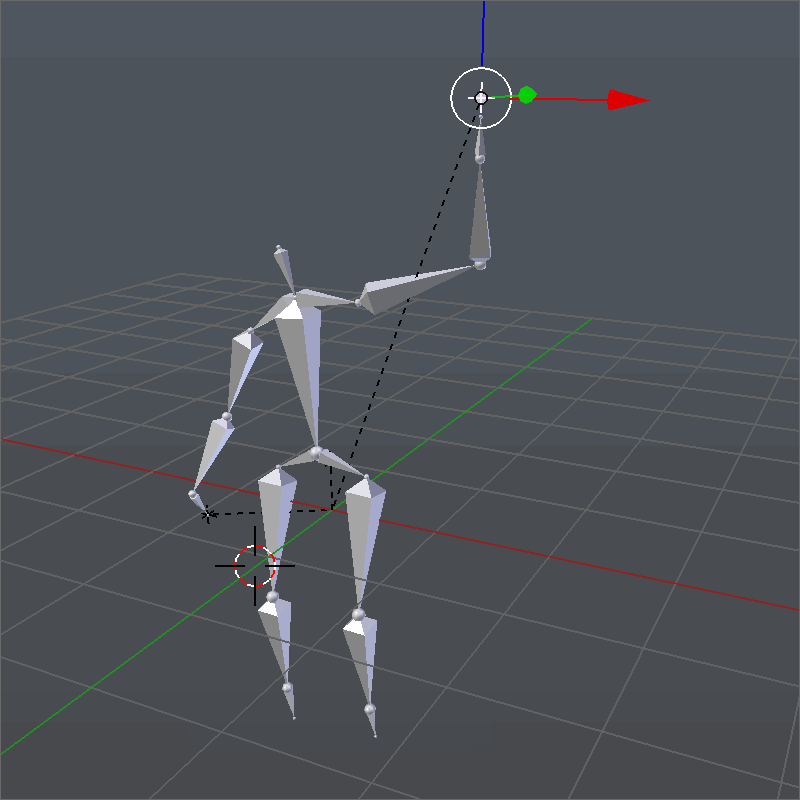
\includegraphics[width=.9\linewidth]{raise-linear-4.png}
    \end{subfigure}

    \caption{A comparison of polar interpolation about the center of mass (top row) and linear interpolation (bottom row) of the control point.}
    \label{img:raise}
\end{figure*}

As a final example, consider the following frames of a sitting animation created with PhysIK with only a single moving control point and 4 static control points figure \ref{img:sit}. 

\begin{figure*}
    \centering
    \begin{subfigure}{0.2\textwidth}
        \centering
        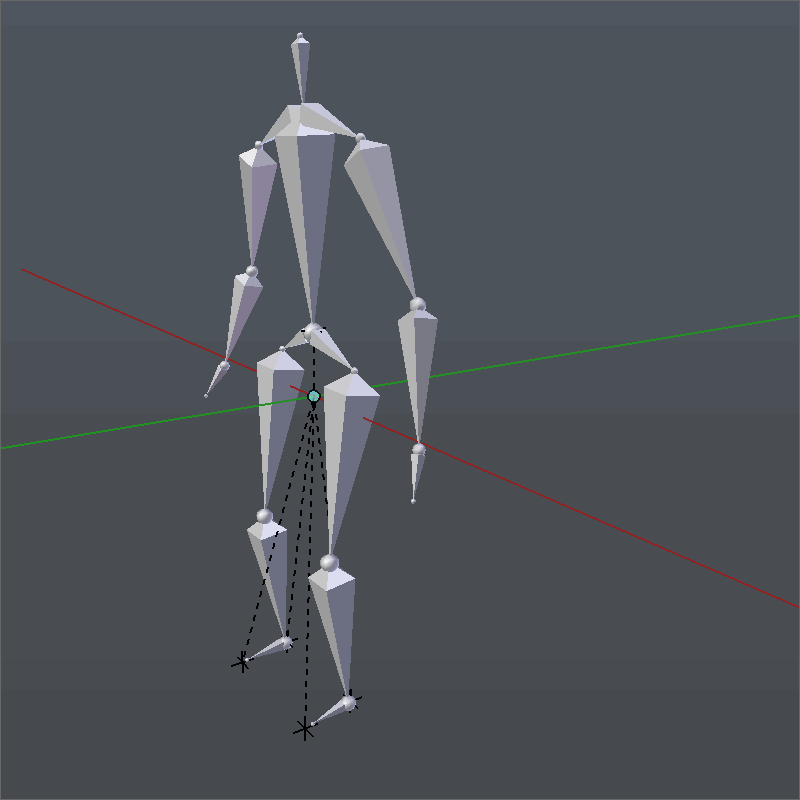
\includegraphics[width=.9\linewidth]{sit-0.png}
        \caption{step 0, $t=0$s}
    \end{subfigure}\begin{subfigure}{0.2\textwidth}
        \centering
        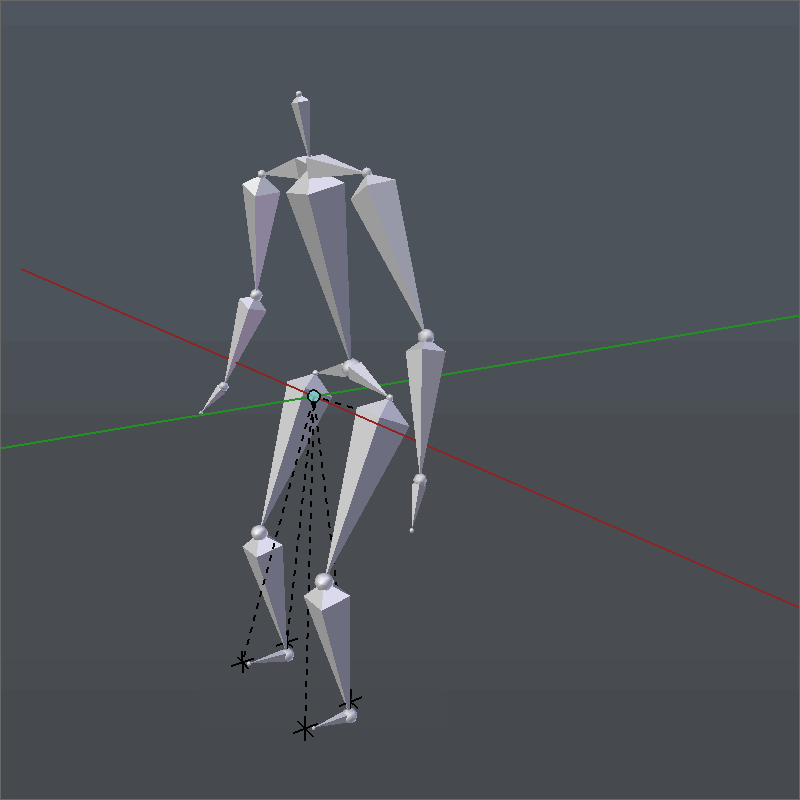
\includegraphics[width=.9\linewidth]{sit-1.png}
        \caption{step 40, $t=1$s}
    \end{subfigure}\begin{subfigure}{0.2\textwidth}
        \centering
        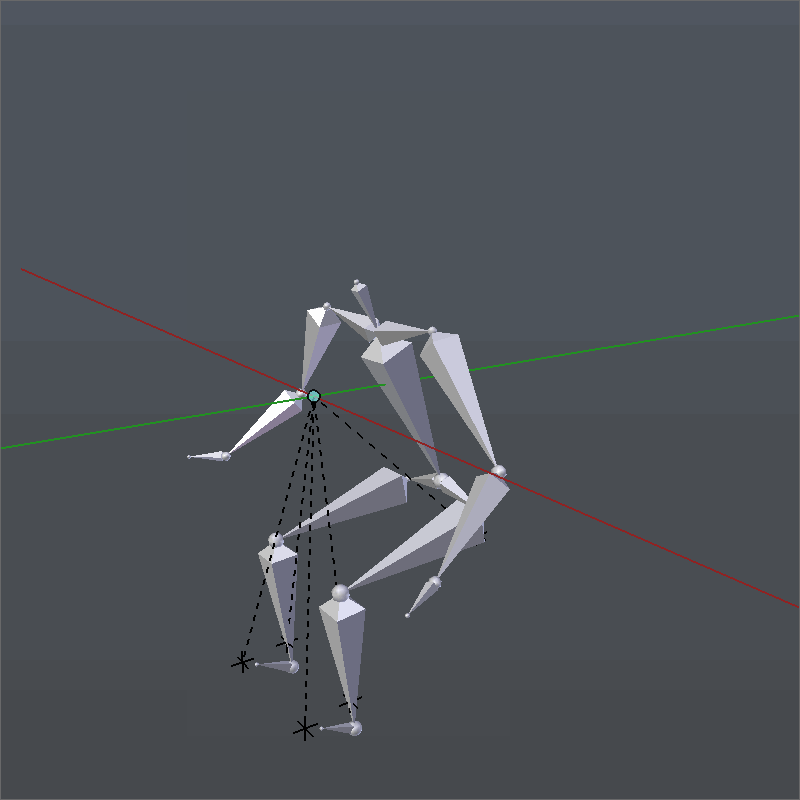
\includegraphics[width=.9\linewidth]{sit-2.png}
        \caption{step 80, $t=2$s}
    \end{subfigure}\begin{subfigure}{0.2\textwidth}
        \centering
        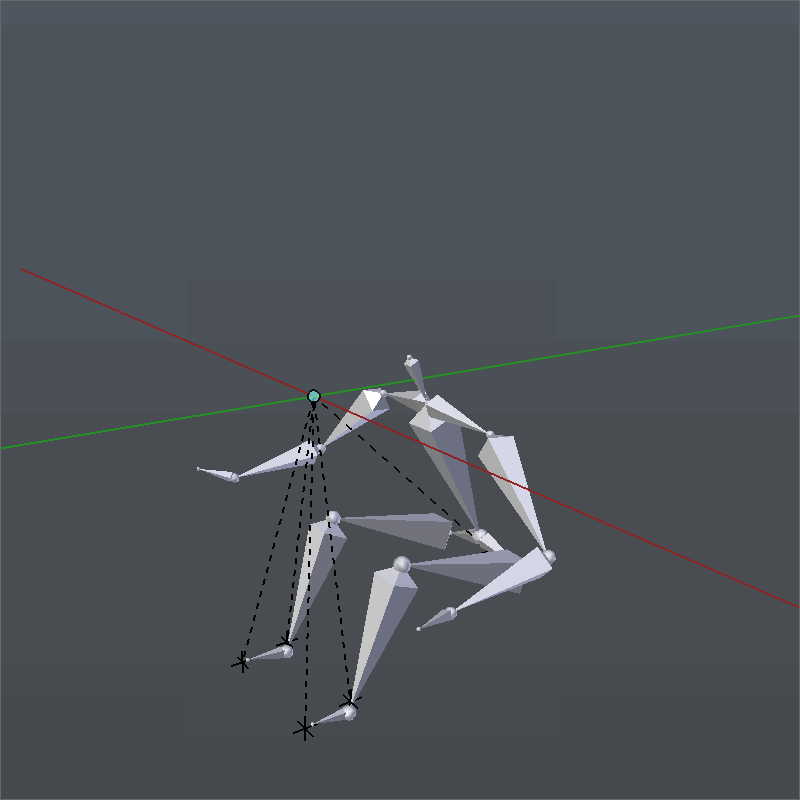
\includegraphics[width=.9\linewidth]{sit-3.png}
        \caption{step 120, $t=3$s}
    \end{subfigure}\begin{subfigure}{0.2\textwidth}
        \centering
        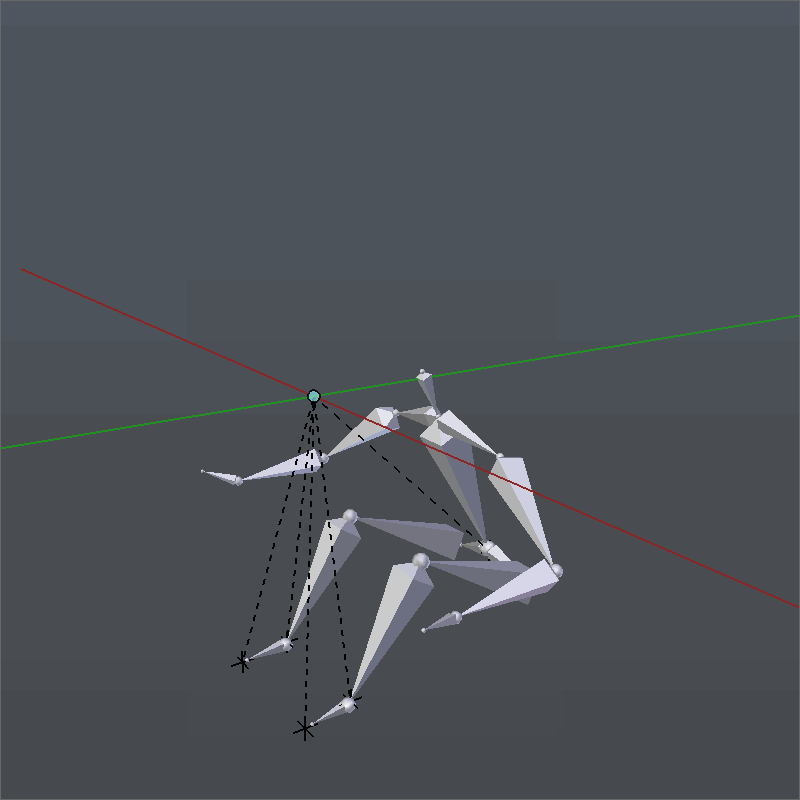
\includegraphics[width=.9\linewidth]{sit-4.png}
        \caption{step 160, $t=4$s}
    \end{subfigure}

    \caption{Frames of a sitting animation}
    \label{img:sit}
\end{figure*}

\section{Discussion \& Future Work}

PhysIK makes it easier to create poses from scratch, with interactive simulations and force-based posing making the who process of posing and animating more intuitive. By simulating external forces, PhysIK mimics the action of posing a wooden mannequin, resulting in natural poses with plausible secondary motion, even with a small number of control points. It does, of course, have its limitations.

The physical simulation in PhysIK can be sensitive to a change in the damping coefficient. If the damping coefficient is too large, then with the Euler's method integration used in this paper, any slight movement is over-corrected, and the resulting oscillations diverge, rendering the tool useless. Too small, and the simulation takes too long to converge. The ideal range of values for the damping coefficient depends on the scale of the model and the mass of each bone. A way to automatically compute the ideal damping coefficient or a different method of damping altogether would help to make the tool even more intuitive. 

PhysIK also breaks down when there are too many tight angular constraints which create a lot of torsion forces. For example, consider a hand, where the carpals are highly constrained in their relative rotations with the metacarpals, which are in turn highly constrained in their relative rotations to the wrist, or root node. Small perturbations tend to be amplified by errors in integration, and any attempt to modify the rig using control points causes the rig to explode. Perhaps better methods of integration or enforcing angular constraints can be explored to mitigate this issue.

PhysIK can also be slow. It may not be desirable to have to wait for the rig to converge onto its target points. In this case, it may be beneficial to pair the physical simulation with CCD or some other fast IK solver. The challenge here would be figuring out when to stop the physical simulation and switch over to the other solver.

\bibliography{research}
\bibliographystyle{ieeetr}

\end{document}